\documentclass{beamer}

\usepackage{graphicx,pdflscape}
\usepackage{xcolor}
\usepackage{changepage}

% \usepackage{forest,adjustbox}
% \useforestlibrary{linguistics}
% \forestapplylibrarydefaults{linguistics}

\usepackage{color}
\usepackage{tikzsymbols}
\usepackage{textcomp}
\usepackage{relsize}
\usepackage{url}

\setbeamercolor{footline}{fg=white}
\setbeamerfont{footline}{series=\bfseries}
\setbeamerfont{footline}{size=\larger}


\title{Introdução a NLP e IR}
\author{Alexandre Rademaker\thanks{Olga Zamaraeva, University of Washington}}
\institute{FGV/EMAp}
\subtitle{Language Models}

\begin{document}
   
\begin{frame}
  \maketitle
\end{frame}

\section{Introduction}

\begin{frame}{Lecture goals}
  \begin{itemize}
  \item Define what language models are
  \item LMs and knowledge
  \item Consider N-gram models as the simplest LM
    \begin{itemize}
    \item Cheap but rigid
    \item The simple math behind N-gram models
    \item Intrinsic evaluation of N-grams (perplexity)
    \end{itemize}
  \item Preview of neural models
    \begin{itemize}
    \item Flexible but expensive
    \item High-level architecture (input, output)
    \item Mention word embeddings as the ``byproduct'' of neural models
    \end{itemize}
  \end{itemize}
  
\end{frame}


\begin{frame}{Language Models: It's all about sequences}

{\it ``A grammar is better, but in practice people use language models.''}
\begin{flushright}
D. Jurafsky
\end{flushright}

\vspace{0.6 cm}

{\it ``You are uniformly charming!'' cried he, with a smile of associating and now
and then I bowed and they perceived a chaise and four to wish for.}
%\vspace{0.5cm}
\begin{flushright}
{\footnotesize Generated by a trigram LM trained on Austen's books}
\end{flushright}

\vspace{0.6 cm}

{\it ``What comes out of a 4-gram model of Shakespeare looks like Shakespeare because it is Shakespeare.'' } 
%\vspace{1 cm}
\begin{flushright}
D. Jurafsky
\end{flushright}
\end{frame}

\begin{frame}{But wait!}

  Haven't we been studying ``language models'' all along? (FSA, FST?)

  \begin{itemize}
  \item Yes and no.
  \item We've been modeling languages with FSA:
    \begin{itemize}
    \item Regular languages
    \item Morphology and phonology
    \item Based on linguistic knowledge
    \end{itemize}
  \item {\it Language Models} is also a {\bf term} denoting a particular kind of statistical models
    \begin{itemize}
    \item We now begin to talk about modeling {\it syntax}*
    \item (though not really; it is about {\it word order} which is a shallower notion than syntax)
    \end{itemize}
  \end{itemize}
\end{frame}

\section{Statistical language models}

\begin{frame}{Language Models}
  
  {\it London is the capital of ...}

  \vspace{0.5cm}

  \begin{itemize}
  \item Language models are programs which output the most probable word given some context
    \begin{itemize}
      \pause
    \item That's it!
    \end{itemize}
    \pause
  \item They output a probability {\it distribution} over the vocabulary
    \pause
  \item ... {\bf N-grams} are the simplest LM: what's the most probable {\bf next} word given a sequence?
    \begin{itemize}
    \item E.g.\ how likely is it that the next word after {\it London is the capital of} is {\it England}? {\it fashion}? {\it swims}?
    \end{itemize}
  \item How would a language model rank the probabilities? 
  \end{itemize}
\end{frame}


\begin{frame}{Statistical Language Models (LM)}
  \begin{itemize}
  \item A notion of modeling language based on e.g.\ word frequencies
  \item Count how many times you saw X follow Y
  \item Now, predict that X will follow Y {\it with some probability}
    \begin{itemize}
    \item {\it London is the capital of} can be plausibly followed by {\it England, the, fashion...}
    \item LM is somewhat creative (the seed {\it was the capital of} may result in a different highest ranked predicted word)
    \end{itemize}
  \item LMs proved to be useful
  \item But are they meaningful?
  \end{itemize}
\end{frame}

\begin{frame}{LMs and linguistic knowledge}
  \begin{itemize}
  \item Statistical and neural LMs are very successful in NLP
  \item They capture some {\bf surface} information about the language (including the ``world knowledge'' that is on the surface)
  \item What about deeper structure, explanations, reasons of phenomena?
\end{itemize}
\end{frame}


\begin{frame}{(Beyond LMs) The role of statistics}

  \begin{footnotesize}
    \url{https://www.tor.com/2011/06/21/norvig-vs-chomsky-and-the-fight-for-the-future-of-ai/} (Kevin Gold's overview)
  \end{footnotesize}

  \begin{center}
    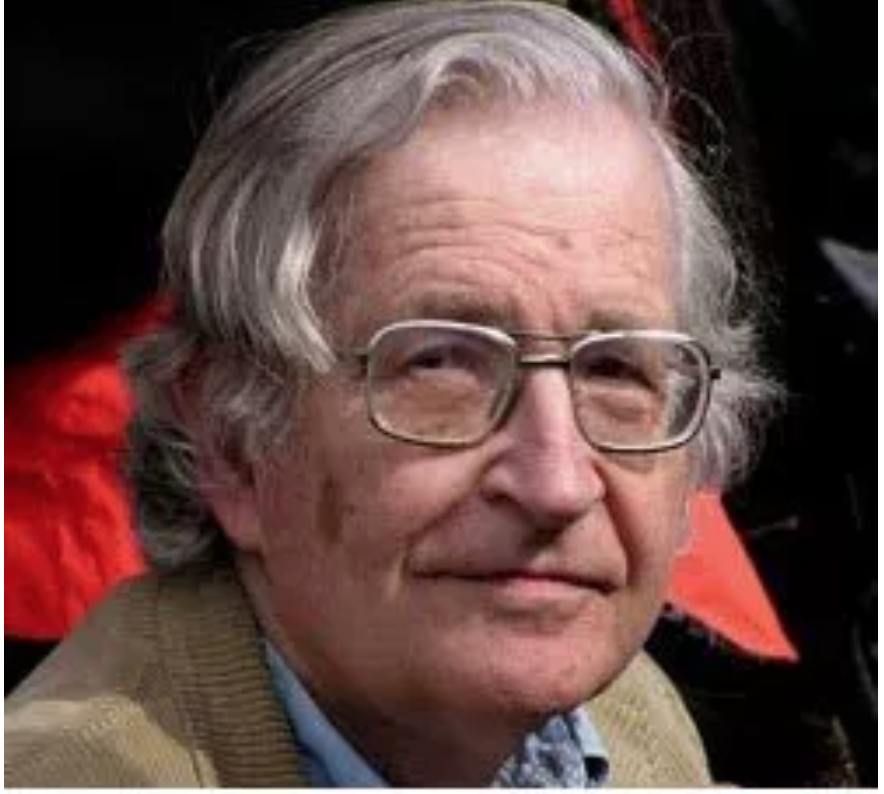
\includegraphics[height=0.3\textheight]{figures/chomsky}
  \end{center}

  Chomsky: {\it To produce a statistically based simulation of ... a
    [bee] dance without attempting to understand why the bee behaved
    that way... is ...a notion of [scientific] success that's very
    novel. I don't know of anything like it in the history of
    science.}
\end{frame}


\begin{frame}{The role of statistics}

  \begin{footnotesize}
    \url{https://www.tor.com/2011/06/21/norvig-vs-chomsky-and-the-fight-for-the-future-of-ai/} (Kevin Gold's overview)
  \end{footnotesize}

  \begin{center}
    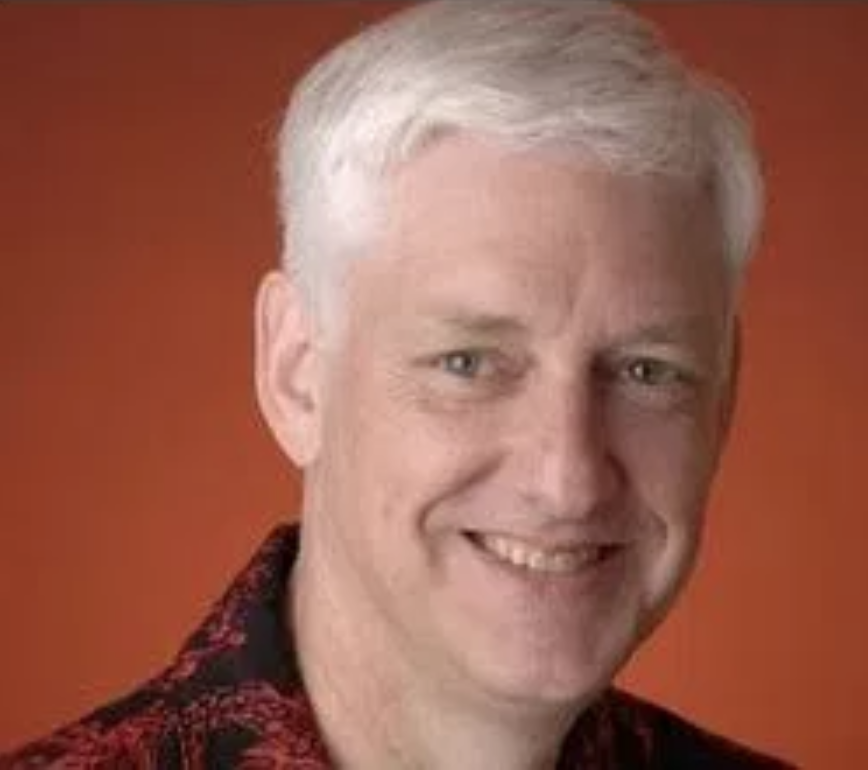
\includegraphics[height=0.3\textheight]{figures/norvig}
  \end{center}

  Norvig: {\it Engineering success correlates with scientific success} 

\end{frame}


\begin{frame}{When are LMs useful?}
  \begin{center}
    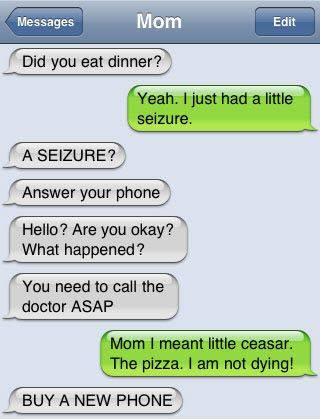
\includegraphics[height=0.4\textheight]{figures/autocorrect}
  \end{center}
  \begin{itemize}
  \item Close captioning (Automatic Speech Recognition)
  \item Easier communication during travel (Machine Translation)
  \item Spelling correction and predictive text
  \item Document classification 
  \end{itemize}
\end{frame}

%\begin{frame}{Text generation (Lab)}
%
%{\it ``You are uniformly charming!'' cried he, with a smile of associating and now
%and then I bowed and they perceived a chaise and four to wish for.}
%
%\begin{flushright}
%{\small Text generated by a trigram language model trained on Jane Austen's books}
%\end{flushright}
%
%%\vspace{0.2cm}
%
%\begin{itemize}
%    \item Classic NLP task
%    \item Fun for homework
%    \item But where is it actually useful?
%    % \begin{itemize}
%    % \item Maybe: create product descriptions automatically
%    % \item ...or word problems for exams
%    % \end{itemize}
%    % \item More generally, machines composing various documents:
%    % \begin{itemize}
%    %     \item What are some ethical implications of that?
%    % \end{itemize}
%    % \item Technique: 
%    % \begin{itemize}
%    %     \item Train an LM on some corpus
%    %     \item Seed the LM with some text for it to start with
%    %     \item Observe it generate text
%    %     \begin{itemize}
%    %         \item ...which will be based on what the LM thinks is most probable continuation for the seed
%    %     \end{itemize}
%    % \end{itemize}
%\end{itemize}
%    
%\end{frame}

\begin{frame}{Main idea behind LMs}
  \begin{itemize}
  \item The LM is {\it trained} on a corpus and can then assign probabilities to new, {\it test} sentences
  \item Train by estimating actual probabilities of word sequences from actual corpora
  \item Then, deploy the model to:
    \begin{itemize}
    \item classify documents in terms of: topic, style, authorship... 
      \begin{itemize}
      \item (which is closer to which model? Is this more like Plato or more like Aristotle?)
      \item (which model says the text is more {\it probable}, according to it?)
      \end{itemize}    	
    \item generate {\it new} text
    \end{itemize}	
  \end{itemize}
\end{frame}

\begin{frame}{N-grams: The (simplified) math behind the simplest LM}

  E.g.\ what probability will a LM trained on corpus TC assign to the
  sentence:

  \vspace{0.2cm}

  {\it ``London is the capital of England''}

  In corpus TC, how many times did we see {\it England} after {\it
    London is the capital of}?

  \vspace{0.2cm}

  $\frac{C(London,is,the,capital,of,England)}{C(London,is,the,capital,of)}$

\end{frame}

% \begin{frame}
% \frametitle{Chain rule of probability}
% \begin{itemize}
% \item Recall the definition of conditional probabilities
% \begin{itemize}
% \item $P(B \vert A) = $
% \item Therefore: $P(A,B) = $
% \end{itemize}
% \item With more variables:
% \begin{itemize}
% \item $P(A,B,C,D) = $
% \end{itemize}
% \item The Chain Rule in General:
% \end{itemize}

% $P(x_1, x_2, x_3, ... x_n) = $

% \vspace{0.5cm}

% P(``London is the capital of England'') =
% 	P(London) x P(is$\vert$London) x  P(the$\vert$London is) 
%          x  P(capital$\vert$London is the) x  P(of$\vert$London is the capital) x P(England$\vert$London is the capital of)

% \end{frame}

% \begin{frame}
% \frametitle{Chain rule of probability}
% \begin{itemize}
% \item Recall the definition of conditional probabilities
% \begin{itemize}
% \item $P(B\vert A) = \frac{P(A,B)}{P(A)}$
% \item Therefore: $P(A,B) = P(B\vert A)P(A)$
% \end{itemize}
% \item With more variables:
% \begin{itemize}
% \item $P(A,B,C,D) = P(A)P(B\vert A)P(C\vert A,B)P(D)P(A,B,C)$
% \end{itemize}
% \item The Chain Rule in General:
% \end{itemize}

% $P(x_1, x_2, x_3, ... x_n) = P(x_1)P(x_2\vert x_1)P(x_3\vert x_1,x_2) ... P(x_n\vert x_1,... x_{n_1})$

% \vspace{0.5cm}

% P(``London is the capital of England'') =
% 	P(London) x P(is$\vert$London) x  P(the$\vert$London is) 
%          x  P(capital$\vert$London is the) x  P(of$\vert$London is the capital) x P(England$\vert$London is the capital of)

% %P(``its water is so transparent'') =
% %	P(its) x P(water$\vert$its) x  P(is$\vert$its water) 
% %         x  P(so$\vert$its water is) x  P(transparent$\vert$its water is so)

% \end{frame}

\begin{frame}
\frametitle{N-grams: The simplest LM}
{\it London is the capital of England}

\vspace{0.3cm}

\begin{itemize}
\item What we'd like to calculate:
\end{itemize}
\begin{center}
	$\frac{C(London,is,the,capital,of,England)}{C(London,is,the,capital,of)}$
%$P(w_1^n) = P(w_1)P(w_2\vert w_1)P(w_3\vert w_1^2)...P(w_n\vert w_1^{n-1}) =$

 %\vspace{0.2cm}

%$ =\prod_{k=1}^{n}P(w_k\vert w_1^{k-1})$


\end{center}
\begin{itemize}
%\pause
\item In some cases, it is possible (using e.g.\ the web)
%\pause
\item But in most cases, we'd never find a corpus big enough
\begin{itemize}
%\pause
%\item How many possible sentences are there in any language?
\item E.g.\ What if I want to know the probability of the sentence {\it Causton is the capital of murder in England}?
\end{itemize}
\end{itemize}
\end{frame}



% \begin{frame}
% \frametitle{Simple (unsmoothed) N-grams}
% \begin{itemize}
% \item What would be the joint probability of ``its water is so transparent that the''?
% \begin{itemize}
% \item We won't find enough occurrences of most (long) real-life sentences
% \end{itemize}
% \end{itemize}
% \end{frame}

% \begin{frame}{N-grams}
%     Not ideal to have to compute joint probabilities directly:
    
%     \vspace{1cm}
%     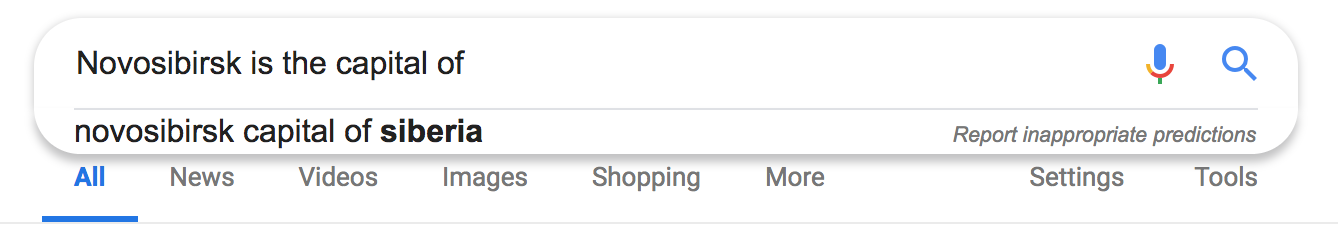
\includegraphics[width=\textwidth]{figures/nsk.png}
% \end{frame}

% \begin{frame}{N-grams}
%     Not ideal to have to compute joint probabilities directly:
    
%     \vspace{1cm}
%     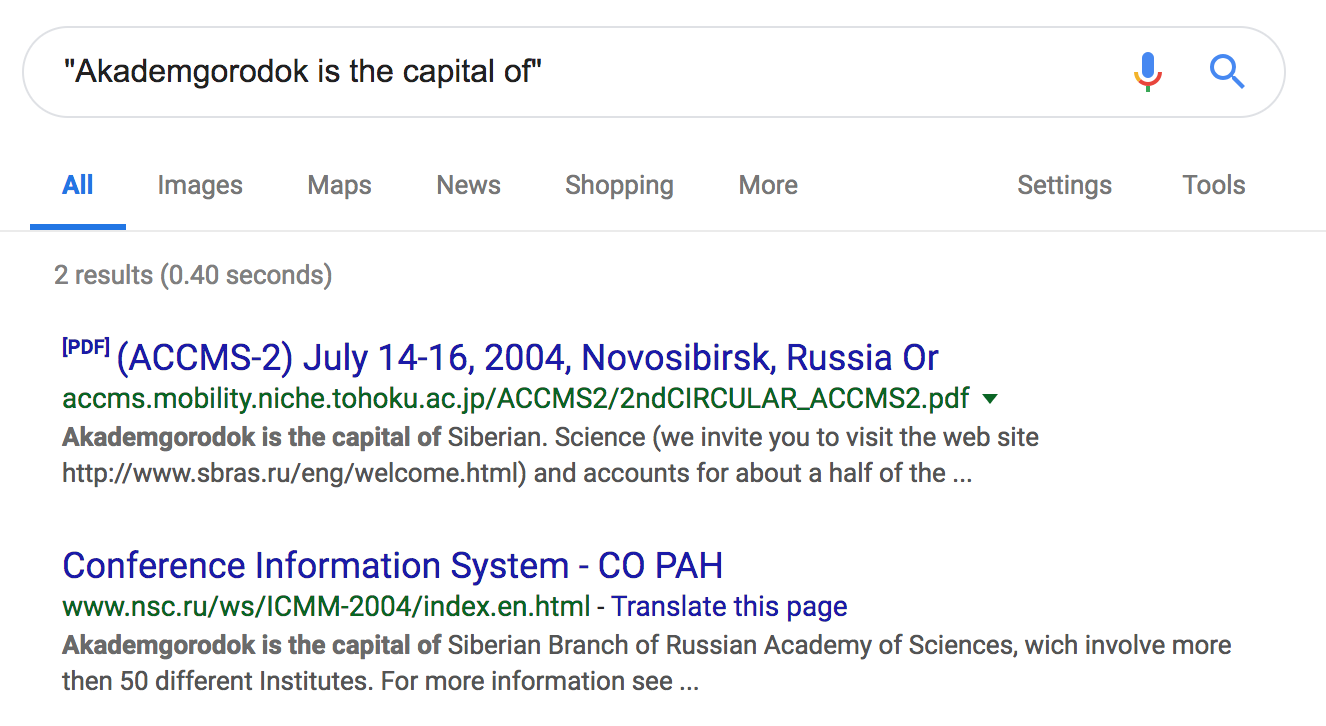
\includegraphics[width=\textwidth]{figures/akadem.png}
%     \end{frame}

\begin{frame}{N-grams: Zero counts}
    Often not {\bf possible} to compute joint probabilities directly:
    
    \vspace{1cm}
    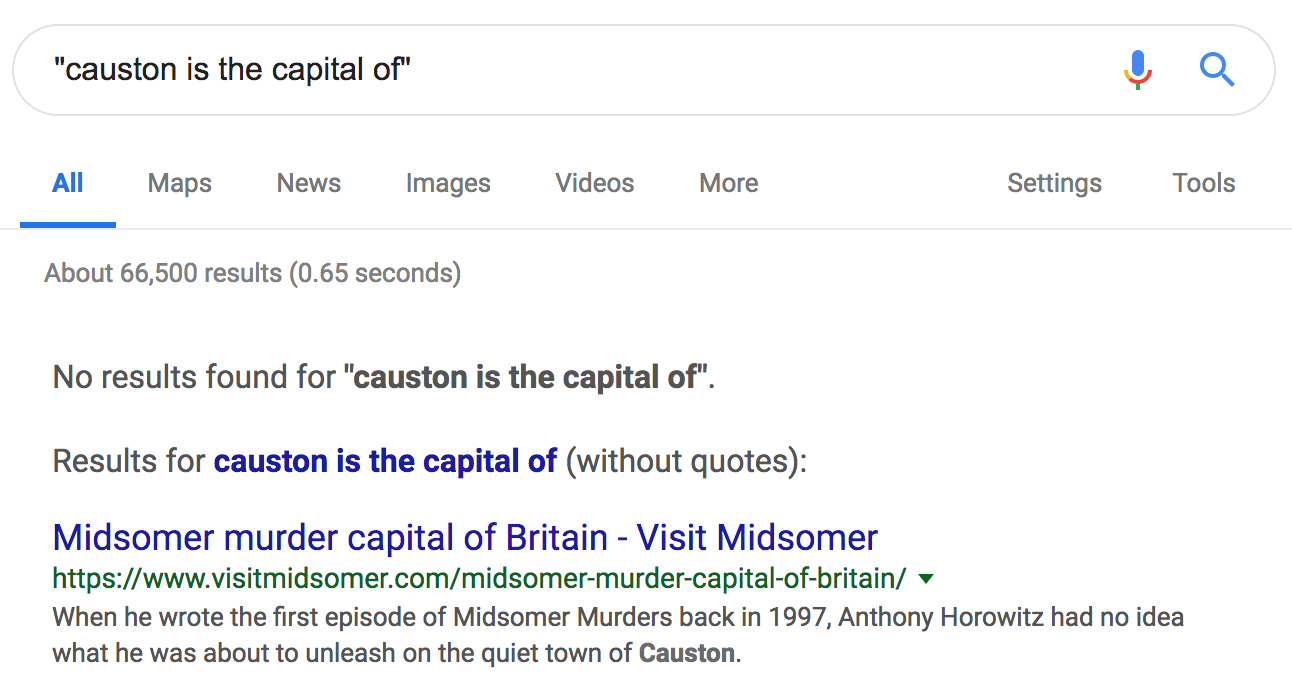
\includegraphics[width=\textwidth]{figures/midsomer.png}
\end{frame}

\begin{frame}
\frametitle{Markov assumption}

\begin{columns}[T] % align columns
\begin{column}{.20\textwidth}
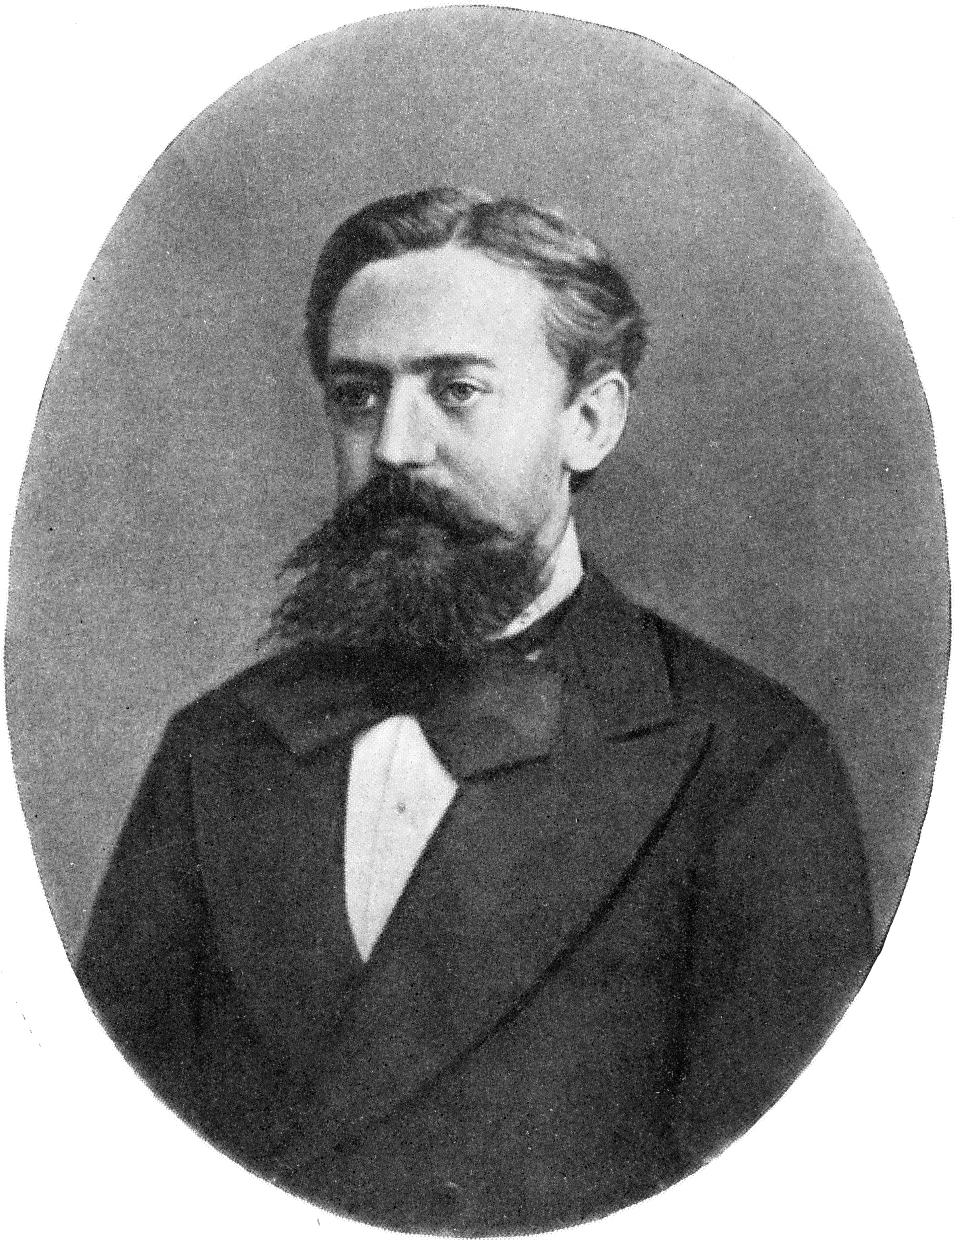
\includegraphics[height=0.2\textheight]{figures/markov.jpg}
\end{column}%
\hfill%
\begin{column}{.75\textwidth}
{\small Andrey Markov (1856-1922)}

{\small (Not-so-fun-fact: In 1908, Markov was fired from the University for refusing to spy on his students)}
\end{column}%
\end{columns}

\vspace{0.5cm}

\begin{itemize}
\item Markov assumption: The probability of a word given a sequence 
only depends on {\bf a few} previous words, not the entire sequence
%\pause
\item {\it Approximate} the history given the last (few) word(s)
\begin{itemize}
\item P(murder$\vert$of), P(of$\vert$capital) instead of P(murder$\vert$capital of)
    \item Will it help me if my corpus does not contain the word {\it Causton}?
\end{itemize}
\end{itemize}

\vspace{0.2cm}

\begin{center}
$P(w_n \vert w_1^{n-1}) \approx P(w_n\vert w_{n-1})$
\end{center}

\vspace{0.5cm}

%\begin{itemize}
%\pause
%\item Is this assumption valid?
%\end{itemize}
\end{frame}

\begin{frame}
\frametitle{N-gram: bigger N means closer approximation}

\begin{itemize}
\item P(England $\vert $London is the capital of)
\begin{itemize}
\item P(England $\vert $of) -- {\bf bigram}
\item P(England $\vert $capital of) -- {\bf trigram}
\item P(England $\vert $the capital of)
\item P(England $\vert $is the capital of)
\end{itemize}
\end{itemize}

\vspace{0.2cm}

\begin{itemize}
    \item Imagine new texts generated by the different models
    \item Is it more useful to be stuck with {\it capital} or {\it is the capital of}?
\end{itemize}

\vspace{0.2cm}



Small N = ``silly'' model, big N = rigid model

\end{frame}

\begin{frame}
\frametitle{N-gram: bigger N means closer approximation}

Consider {\it generating} from such models:

\vspace{0.2cm}

\begin{itemize}
\item P(him $\vert $Alas poor Yorick I knew )
\begin{itemize}
\item P(him $\vert $knew) -- {\bf bigram}
\item P(I $\vert $knew him) -- {\bf trigram}
\item P(Yorik $\vert $I knew him)
\item P(poor $\vert $Yorick I knew him)
\item P(Alas $\vert $poor Yorick I knew him)
\end{itemize}
\end{itemize}

\vspace{1 cm}

Small N = ``silly'' model, big N = rigid model (how interesting is it to generate exact strings from Shakespeare's {\it Hamlet}?)
% {\it ``What comes out of a 4-gram model of Shakespeare looks like Shakespeare because it is Shakespeare.'' } 

% \begin{flushright}
% D. Jurafsky
% \end{flushright}

\end{frame}

 \begin{frame}
 \frametitle{Maximum Likelihood Estimates for bigram counts}
 \begin{itemize}
 \item Bigram probability for a word y given a previous word x: 
 \item Out of all the times you saw x, in what percentage was it followed by y?
 \end{itemize}

 \vspace{0.5cm}

 \begin{center}
 $P(w_n\vert w_{n-1}) = \frac{C(w_{n-1}w_n)}{C(w_{n-1})}$
 \end{center}
 \end{frame}

 \begin{frame}{Small example (from Jurafsky\&Martin 2008)}

 \begin{itemize}
 \item Out of all the times you saw x, in what percentage was it followed by y?
 \end{itemize}

 \vspace{0.5cm}

 \begin{center}
 $P(w_n\vert w_{n-1}) = \frac{C(w_{n-1}w_n)}{C(w_{n-1})}$
 \end{center}

 \vspace{0.5cm}

 <s> I am Sam </s>

 <s> Sam I am </s>

 <s> I do not like green eggs and ham </s> 

 \vspace{0.5cm}

 P(do $\vert$ I) = 

 \vspace{0.5cm}

 {\small (Respond at: \url{https://pollev.com/olgazamaraev657})}

 \end{frame}

 
 \begin{frame}{Unknown words}
 \begin{itemize}
 \item What would a n-gram model trained as described so far say about the probability of a sentence with an unknown word in it?
 \begin{itemize}
 \pause
 \item To not allow 0 probabilities, anticipate an {\it UNK} word in the vocabulary, assign it some small probability, redistribute the rest of the probabilities so that all probabilities still sum to 1
 \begin{itemize}
     \item ''Smoothing'' (and it does not come for free)
     \item Next lecture
 \end{itemize}
 \end{itemize}
 \end{itemize}
 \end{frame}

\begin{frame}
\frametitle{Probability vs. Frequency}
\begin{itemize}
	\item Probability: How likely something is to happen
	\item Frequency: How frequently something has happened in a set of observations
	\item Probability clearly influences frequency
	\item Frequency can be used to estimate probability 
	\begin{itemize}
		\item ... but they are not the same thing
	\end{itemize}
	\item If a bigram never appears in a training corpus:
	\begin{itemize}
		\item What is its observed frequency?
		\item What is its probability?
	\end{itemize}
\end{itemize}
\end{frame}


\begin{frame}
\frametitle{Exercise: Bigger Example}
\begin{itemize}
\item What are the bigrams in the following mini corpus?  What are their MLEs?
\end{itemize}

{\bf $<$s$>$ How much wood would a wood chuck chuck if a wood chuck 
could chuck wood? $<$/s$>$ $<$s$>$ As much wood as a wood chuck could if a wood chuck could chuck wood. $<$/s$>$ }

\begin{itemize}
\item What probability does that bigram model assign to the following sentences?
\end{itemize}

{\bf $<$s$>$ How much wood. $<$/s$>$}

{\bf$<$s$>$ How much wood? $<$/s$>$}

{\bf$<$s$>$ As much wood chuck chuck chuck wood. $<$/s$>$}

{\bf$<$s$>$ How would a wood chuck chuck ? $<$/s$>$}

\end{frame}

\begin{frame}
\frametitle{Bigrams}
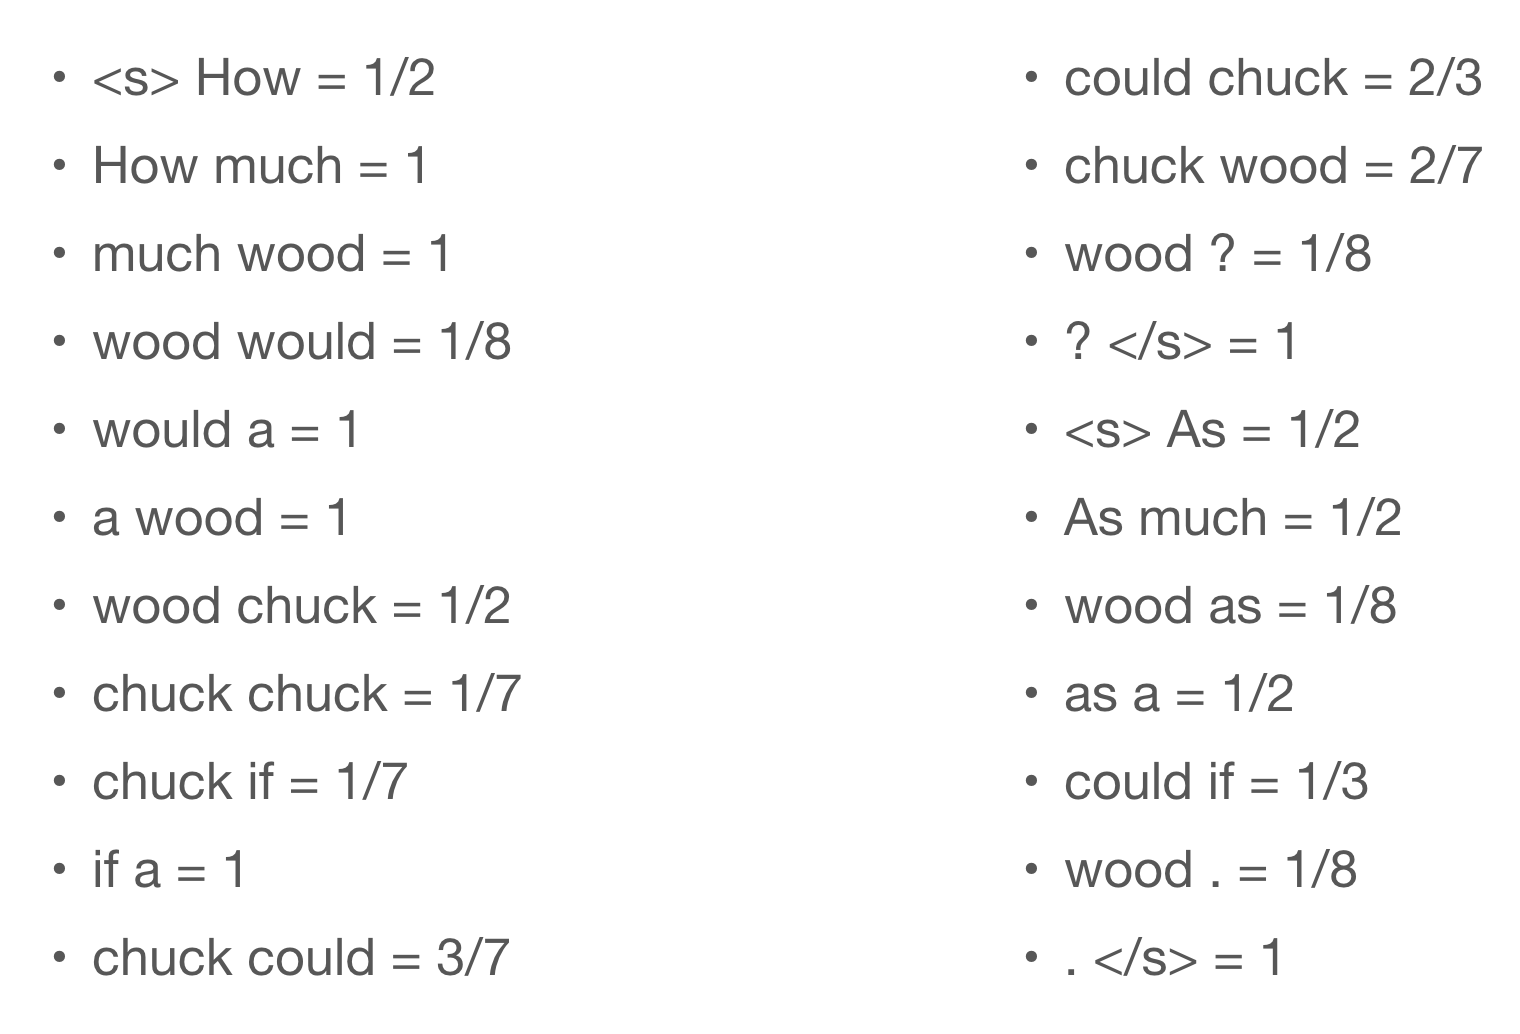
\includegraphics[width=\textwidth]{figures/woodchuck1}
\end{frame}

\begin{frame}
\frametitle{Sentences}
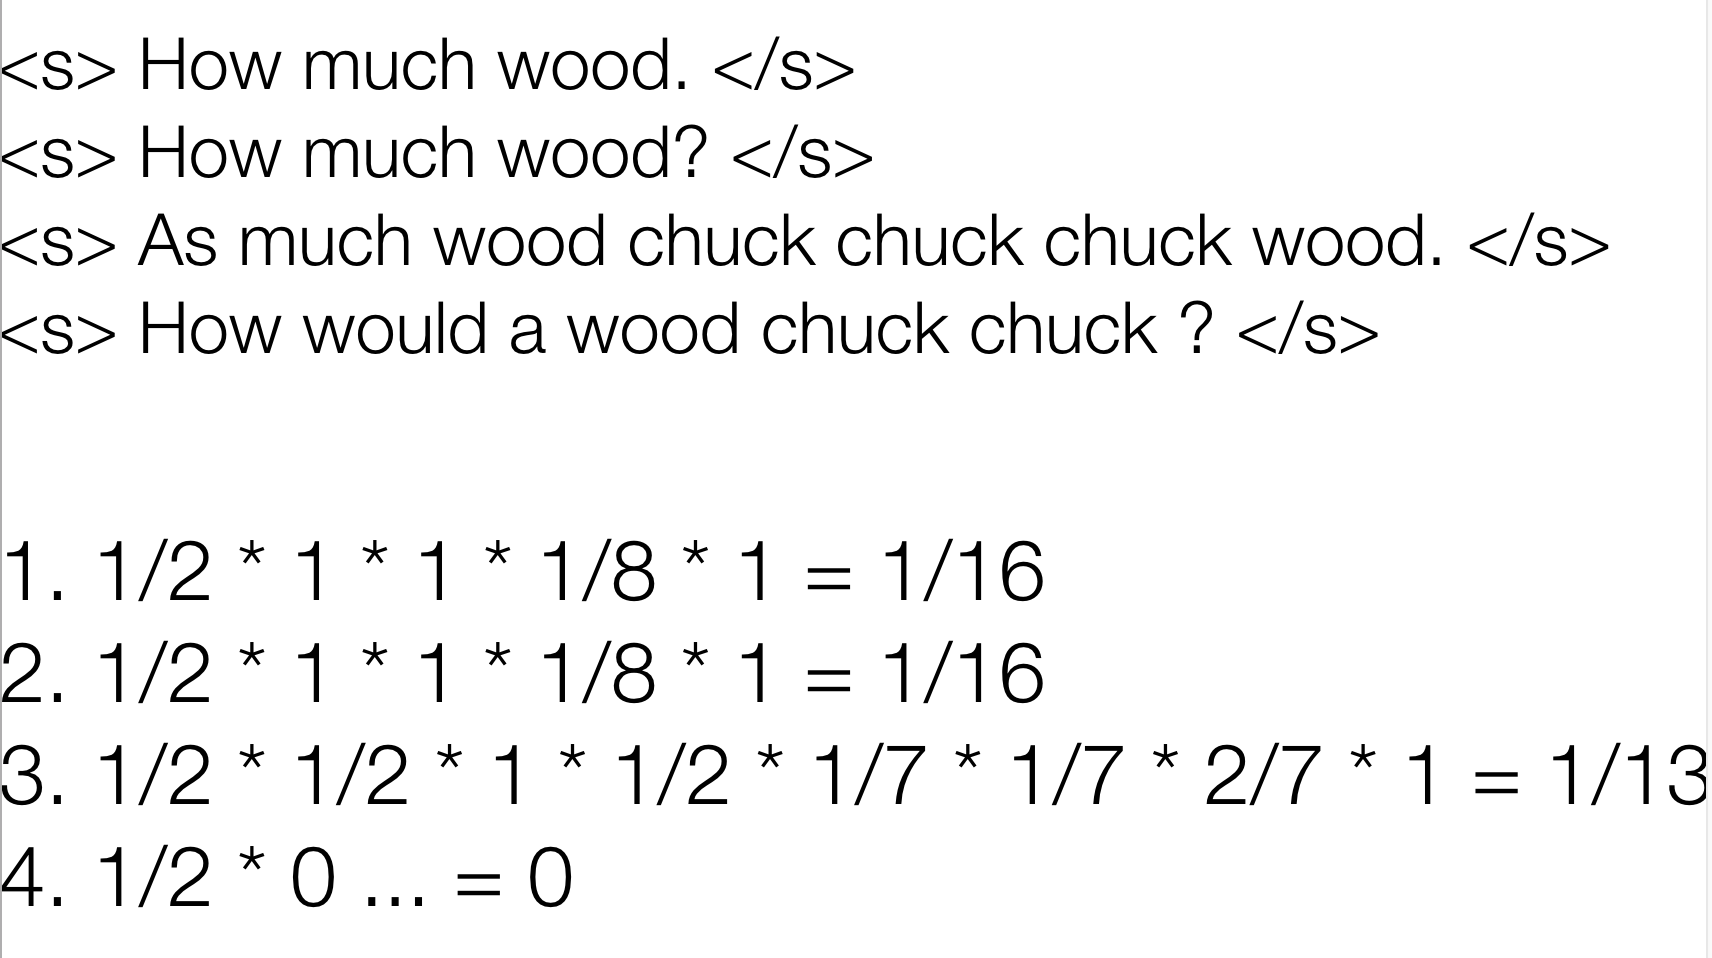
\includegraphics[width=\textwidth]{figures/woodchuck2}
\end{frame}

\begin{frame}
\frametitle{Generating from a N-gram model}
``{\it i had called upon my friend , mr . sherlock holmes , which i should ever communicate to the public .}''

\vspace{0.5cm}

\begin{itemize}
	\item Start with a {\bf seed} sequence of length N
	\item The model outputs the most probable word given the seed
	\item Now the last N-1 words from the seed plus the freshly output word become the {\bf history}
	\item The model outputs the most probable word given history
	\item etc.
\end{itemize}
\end{frame}
\begin{frame}
\frametitle{Counting things in a corpus}
\begin{itemize}
\item Type/token distinction
\item But what counts as a token?  What are some cases where this is not obvious? 
\item And what counts as the same type?  What are some cases where this is not obvious?
\item Is there a single right answer?
\end{itemize}
\end{frame}

\subsection{Tokens and Types}
\begin{frame}
\frametitle{Counting things in a corpus}
\begin{itemize}
\item Type/token distinction
\item But what counts as a token?  What are some cases where this is not obvious? 
\begin{itemize}
\item Contracted forms, punctuation, hyphenated forms, words with spaces (New York), ...
\end{itemize}
\item And what counts as the same type?  What are some cases where this is not obvious?
\begin{itemize}
\item Caps/non-caps, word-form/lemma, homographs, ...
\end{itemize}
Is there a single right answer?
\begin{itemize}
\item No: It depends on the application context
\end{itemize}
\end{itemize}
\end{frame}

\section{Evaluation and Perplexity}
\begin{frame}
\frametitle{Evaluating N-gram models}
\begin{itemize}
\item What kinds of extrinsic evaluation are possible?
\item What kinds of intrinsic evaluation are possible?
\end{itemize}
\end{frame}

\begin{frame}
\frametitle{Evaluating N-gram models}
\begin{itemize}
\item What kinds of extrinsic evaluation are possible?
\begin{itemize}
\item ASR, MT, ...
\end{itemize}
\item What kinds of intrinsic evaluation are possible?
\begin{itemize}
\item Perplexity: Given an n-gram model trained on some training set, how well does it predict the test set? (i.e., what probability does it assign to the test set?)
\end{itemize}
\end{itemize}
\end{frame}


\begin{frame}
\frametitle{Perplexity (intrinsic evaluation)}
\begin{itemize}
\item Which model assigns the {\bf highest probability} to the test set?
\item {\it Perplexity (PP)} is the inverse probability normalized by word count 
\begin{itemize}
\item Informally, how ``surprised'' is the model by the test set?
\item Information theory
\end{itemize}
\item E.g. for a test set $W = w_1w_2w_3...w_N$
\end{itemize}

$PP(W) = P(w_1w_2w_3...w_N)^{\frac{-1}{N}} = (\prod_{i=1}^N{P(w_i\vert w_1...w_{i-1})})^{\frac{-1}{N}}$

\vspace{0.5cm}

$\approx (\prod_{i=1}^N{P(w_i\vert w_{i-1})})^{\frac{-1}{N}}$

\end{frame}

\begin{frame}
\frametitle{Perplexity}

\begin{itemize}
	\item Perplexity can bee seen as an average {\it branching factor} of a language
	\item e.g. consider a language of digits where each digit has a probability of 0.1 of following another digit
\end{itemize}

\vspace{4cm}

Is this high perplexity?

\end{frame}


\begin{frame}
\frametitle{Perplexity}

\begin{itemize}
\item Perplexity can bee seen as an average {\it branching factor} of a language
\item e.g. consider a language of digits where each digit has a probability of 0.1 of following another digit
\end{itemize}

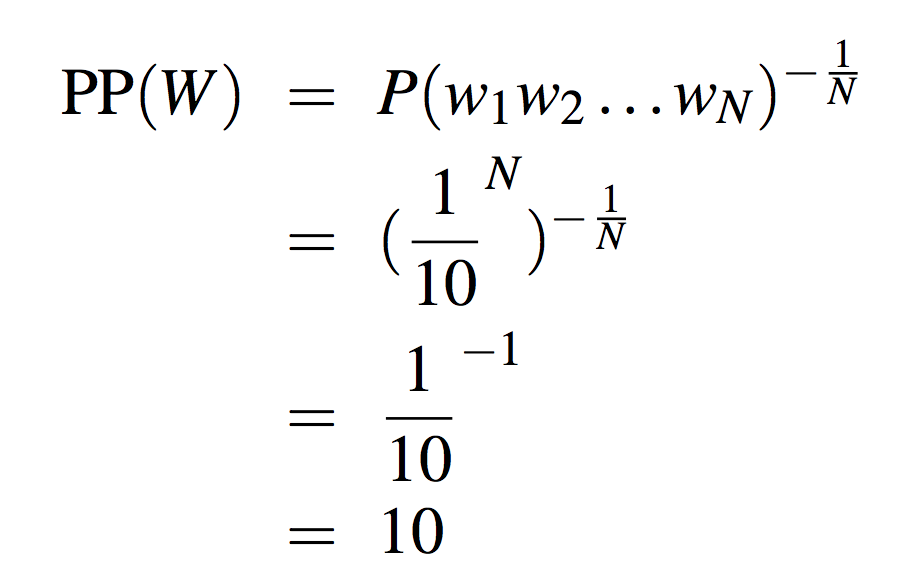
\includegraphics[height=0.5\textheight]{figures/ppl}

Is this high perplexity?

\end{frame}



 \begin{frame}{Other varieties of statistical LMs}
 \begin{itemize}
     \item Hidden Markov Models
     \begin{itemize}
         %\item A kind of weighted Finite State Automata
         \item were widely used in ASR
     \end{itemize}
     \item Probabilistic CFGs
     \begin{itemize}
         \item Assign probabilities to sequences of ``constituents''
         %\item P(NP | Det N) is high
         %\item were widely used in a variety of NLP tasks
     \end{itemize}
     \item ...all of these have similar limitations as n-grams
     \begin{itemize}
         \item (either approximate too little or too much)
     \end{itemize}
 \end{itemize}
 \end{frame}

\begin{frame}{Desireable: Generalizing over contexts}
    \begin{itemize}
        \item {\it London} is the capital of...
        \item {\it Causton} is the capital of...
    \end{itemize}
    
    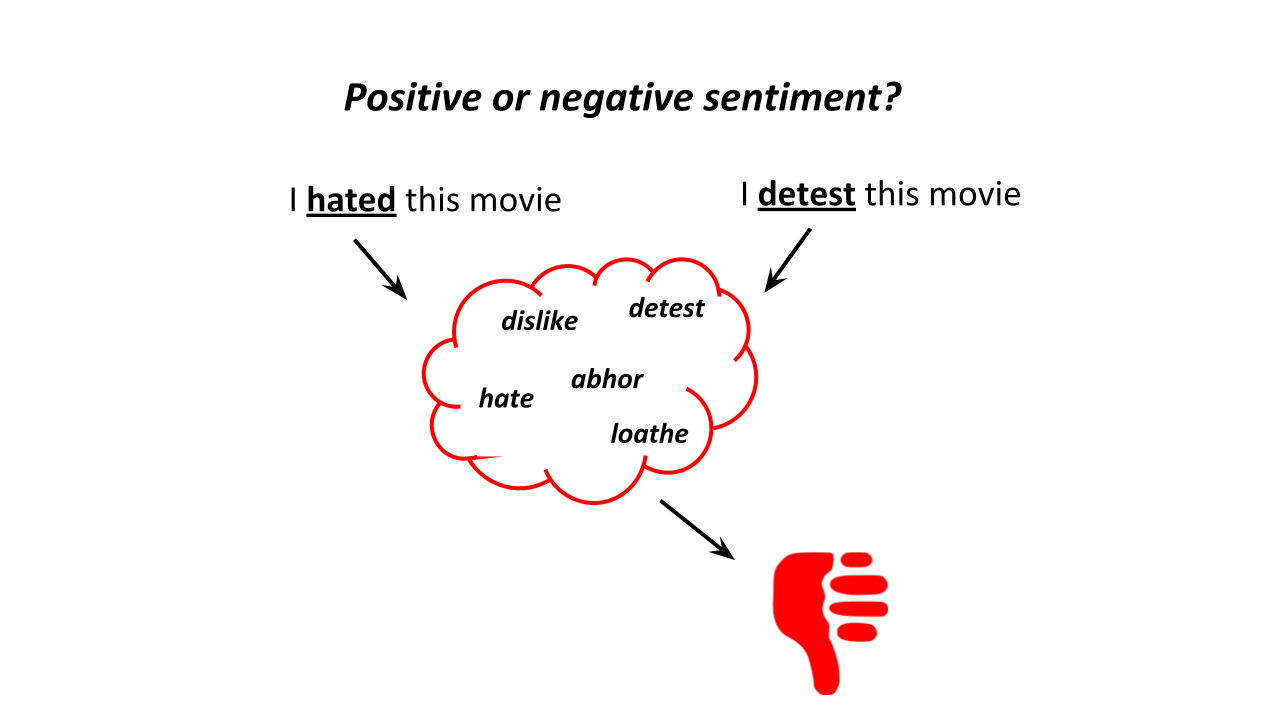
\includegraphics[height=0.5\textheight]{figures/sentiment.png}
    
    {\tiny Figure from Allyson Ettinger's tutorial at SCiL 2019}
\end{frame}


\section{Neural language models (preview)}
\begin{frame}{Neural* language models}
\begin{itemize}
    \item Predict the word given context (or vice versa)
    \item Generalize over contexts, are more ``creative'' than n-grams:
    \begin{itemize}
        \item Learn which words occur in similar contexts
        \item It is possible to build a neural model that creates representations for unknown words ``on the fly''**
    \end{itemize}
    \item But:
    \begin{itemize}
        \item Are more complex to train
        \item Require lots of training data to start working well
        \item Learn the training data biases
    \end{itemize}
\end{itemize}

\vspace{1cm}

{\small *These are {\it simplified} neural architectures}

{\small **Not the same architecture as in the lecture}
\end{frame}


\begin{frame}{(Simplified) neural models architecture}

% \begin{columns}[T] % align columns
% \begin{column}{.20\textwidth}

% \end{column}%
% \end{columns}
\begin{small}
\begin{itemize}
    \item The {\it feed-forward} SkipGram model (Mikolov et al)
    \item Input: a word from the vocabulary
    \item Middle: two matrices and some matrix multiplication
    \item Output: a probability for each word in the vocabulary occurring {\it somewhere nearby} the input word 
\end{itemize}

\end{small}
    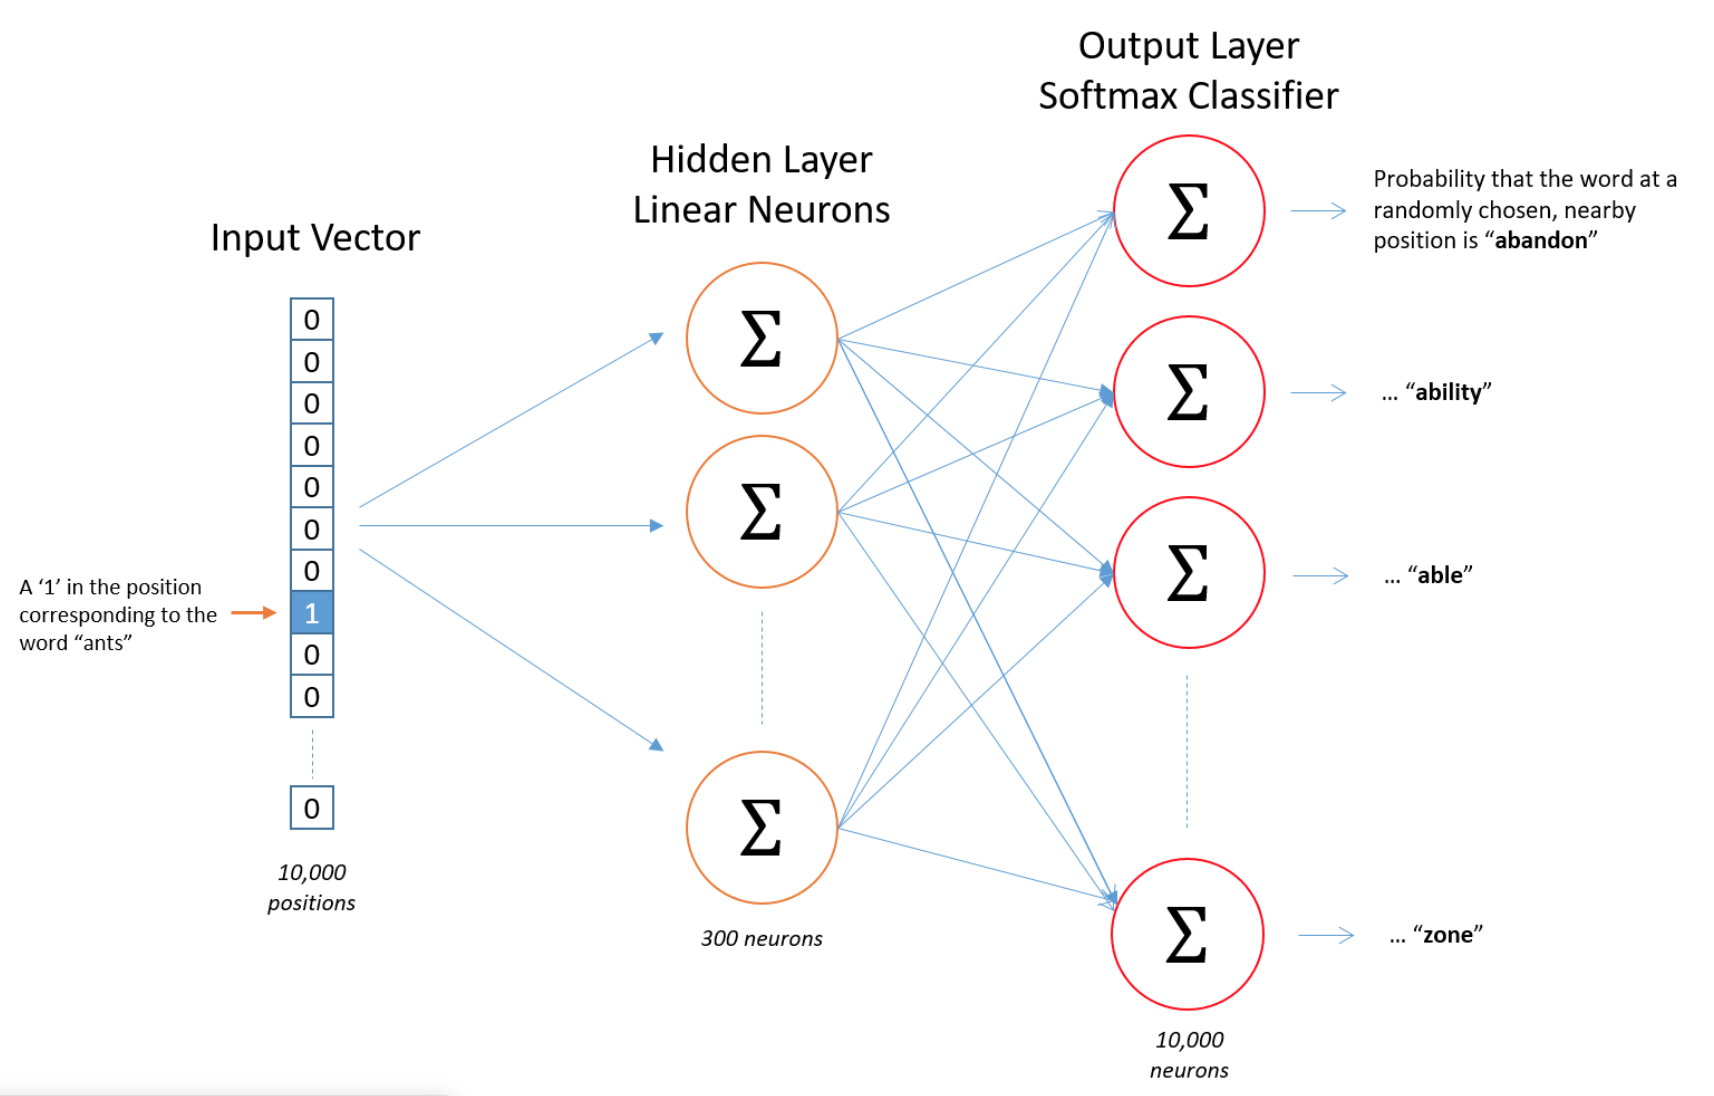
\includegraphics[width=0.8\textwidth]{figures/skipgram1}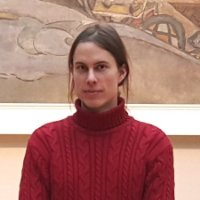
\includegraphics[height=0.2\textheight]{figures/mikolov.jpg}
    
    \tiny{Pic from: \url{http://mccormickml.com/2016/04/19/word2vec-tutorial-the-skip-gram-model/}}
\end{frame}

%\begin{frame}{ML training review}
%
%\begin{itemize}
%\item We said we ``trained'' N-gram models but really we were relying directly on counts, no iterative training required
%    \item Generally in ML: Represent things as {\bf feature vectors} and find some {\bf parameters} for each dimension such that some {\bf computation} leads to a {\bf good enough accuracy}
%    \begin{itemize}
%    %\pause
%        \item E.g.\ learn to distinguishing cats from dogs by representing animals as vectors:
%        \begin{itemize}
%            \item x1 = [meows=1, barks=0, furry=1]
%            \item The system learns that it should mostly output y(is cat?)=1 for vectors that look like x1 
%            %\pause
%            \item The system will probably learn that the weight for ``furry'' should be near 0! (why?) 
%        \end{itemize}
%    \end{itemize}
%    %\pause
%\end{itemize}
%\end{frame}
%
%\begin{frame}{SkipGram training}
%\begin{itemize}
%\item Input: a word
%\item Output: a probability distribution over the vocabulary
%\item {\bf In the middle:} two {\it matrices}, ``features'' and ``weights''
%    %\item Train (simplified) neural networks to predict which words can serve as context to the input word
%    %\pause
%    \begin{itemize}
%    %\pause
%        \item start with some random matrices
%        \item an input word is mapped to {\bf some} vector (matrix row) at the start; call it the word vector
%        \item word vector is multiplied by weight matrix, the output is a vector of probabiltiies
%        %\pause
%        \item iteratively find numbers for {\bf both} the word vectors {\bf and} the weights such that the output probabilities are ``good enough''
%        \item unlike our cat example, the features are {\it learned} in the process along with feature weights
%    \end{itemize}
%  \end{itemize}  
%\end{frame}
%
%% \begin{frame}{Vector space models architecture}
%% \begin{itemize}
%%     \item Based on two components:
%%     \begin{itemize}
%%         \item Represent words as vectors of numeric values, such that {\bf similar words have similar vectors}
%%         \pause
%%         \item (Advanced material) Use {\bf dimensionality reduction} to represent words as {\bf dense vectors}
%%         \begin{itemize}
%%         \item (see additional XOR additional exercise)
%%         \end{itemize}
%%     \end{itemize}
%%     \pause
%%     \item Typically word vectors are {\bf both learned and used} in {\it neural architectures}
%% \end{itemize}
%    
%% \end{frame}
%
%
%% \begin{frame}{Words and contexts}
%% In a real corpus, you will probably see e.g.\ the word {\it Vancouver} (and other BC city names!) ``in the company'' of the word {\it BC} more often than {\it Manitoba}.
%
%% \vspace{0.5cm}
%
%%     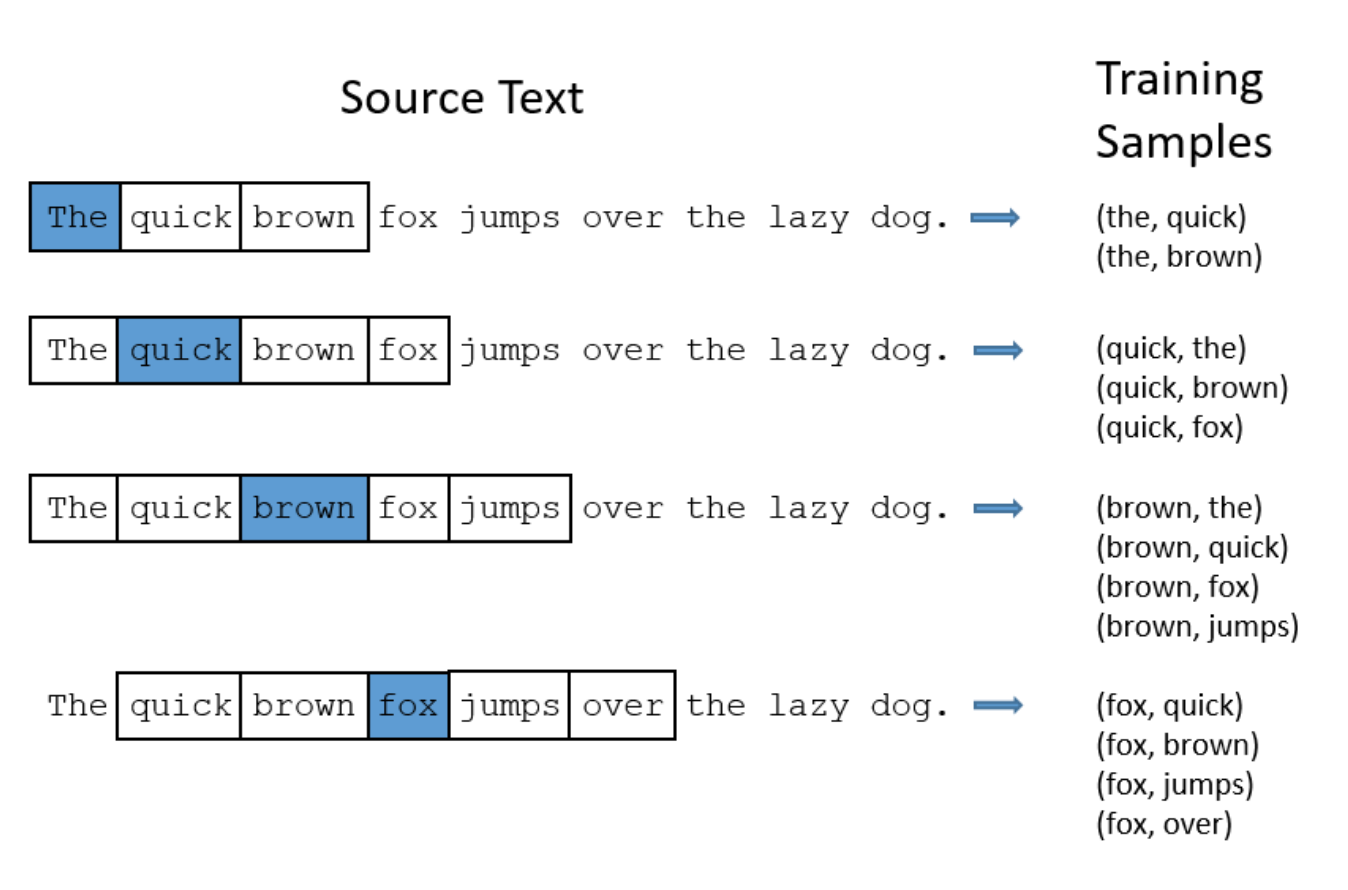
\includegraphics[height=0.6\textheight]{figures/wordpairs}
%
%% \tiny{Pic from: \url{http://mccormickml.com/2016/04/19/word2vec-tutorial-the-skip-gram-model/}}
%% \end{frame}
%
%
%% \begin{frame}{Neural language models and word embeddings}
%
%% Main idea: Given a corpus, find some sets (matrices) of parameter values (weights) so that the probability of the corpus is maximized
%
%% \begin{itemize}
%%     \item exactly the same goal that N-gram models have
%%     \item instead of looking at n-gram sequences:
%%     \begin{itemize}
%%         \item think of words as n-dimensional vectors
%%         \item put together some computational units (e.g.\ in the XOR network, the ReLU units were computing the sum of values (and mapping negative results to 0))
%%         \item find specific values for these vectors and specific weights for each dimension, such that:
%%         \begin{itemize}
%%             \item if you send a vector for word w1, e.g.\ {\it chicken} into the neural pipeline, the output at the very end is a vector of length V (size of the vocabulary) with each value being the probability that the word v occurs next to the input word w1
%%             \item e.g.\ the probability of the word {\it wings} or the word {\it duck} should be high but the probability of the word {\it ocean} may be much lower
%%         \end{itemize}
%%     \end{itemize}
%% \end{itemize}
%    
%%\end{frame}
%
%
%% \begin{frame}{Neural language models and word embeddings}
%% \begin{itemize}
%%     \item Represent words as vectors of numbers of length d
%%     \begin{itemize}
%%         \item d is usually between 50 and 500
%%     \end{itemize}
%%     \item Intuition:
%%     \begin{itemize}
%%         \item Start with a random embedding
%%         \item Iteratively make the embedding more similar to that of the word’s neighbors (so that the dot product is high)
%%     \end{itemize}
%%     \item At the end, we have a {\it language model} which predicts the word's context (or the context, given word)
%%     \begin{itemize}
%%         \item In practice, these are often discarded and it is only the resulting embeddings that people are interested in
%%         \begin{itemize}
%%             \item ...to use in various architectures for the same core set of NLP tasks
%%         \end{itemize}
%%     \end{itemize}
%% \end{itemize}
%% \end{frame}
%
%% \begin{frame}{Neural networks: Training for high cosine}
%
%% ``Similar vectors'': the cosine similarity (the dot product)
%
%% \vspace{0.5cm}
%
%% 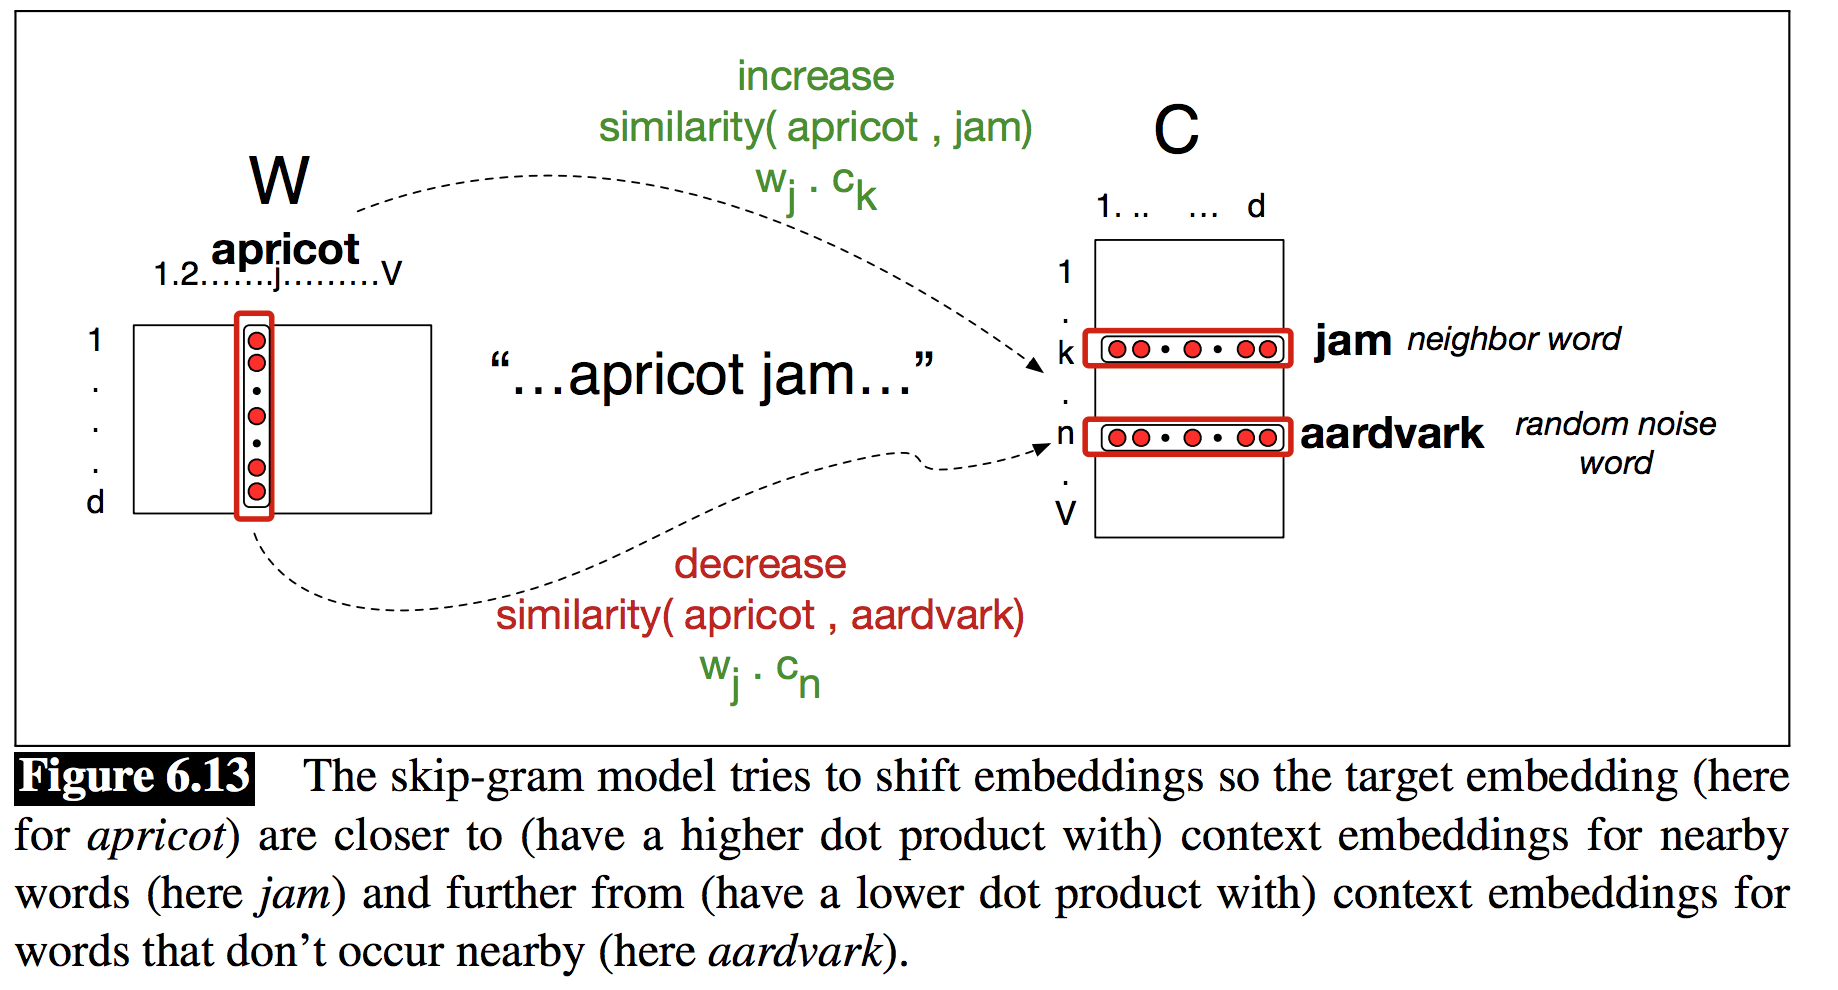
\includegraphics[width=\textwidth]{figures/apricot}
%% \end{frame}
%
%\begin{frame}{The SkipGram model in training}
%
%\small{The e.g.\ orange output vector contains likelihood scores for each of the words in the vocabulary occurring 2 words before the word ``tape''}
%
%\begin{minipage}{0.6\textwidth}
%    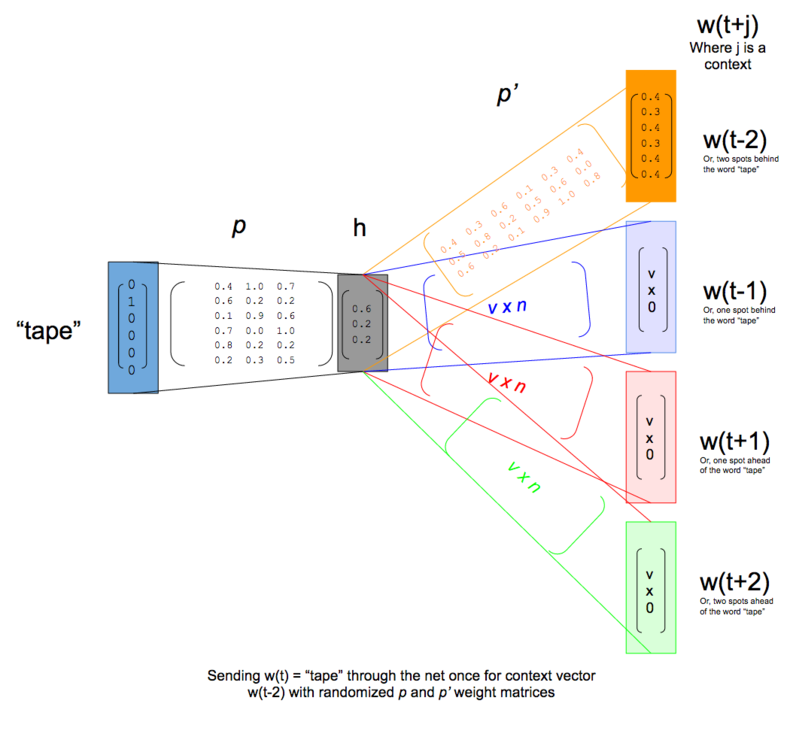
\includegraphics[width=\textwidth]{figures/skip-gram} 
%\end{minipage}
%\begin{minipage}{0.3\textwidth}
%\begin{itemize}
%    \item computation is the {\it dot product}: $p \cdot h$, $h \cdot p'$
%    \item (p' has to be transposed)
%    \item then need to map likelihood scores to actual probabilities (e.g.\ {\it softmax})
%\end{itemize}
%\end{minipage}
%    
%    \tiny{Pic from: \url{https://medium.com/district-data-labs/forward-propagation-building-a-skip-gram-net-from-the-ground-up-9578814b221}}
%\end{frame}
%
%% \begin{frame}{Words and contexts, recap}
%
%% \begin{small}
%% Assume a corpus which contained lots of instances of {\it quick brown fox} but also {\it quick brown dog}. There are {\bf two levels} of generalization here:
%% \end{small}
%
%% \begin{itemize}
%%     \item The word {\it quick} will end up close to the words {\it dog} and {\it fox} in the vector space
%%     \item The words {\it dog} and {\it fox} will end up close to each other, too!
%% \end{itemize}
%
%%  \vspace{0.2cm}
%
%%     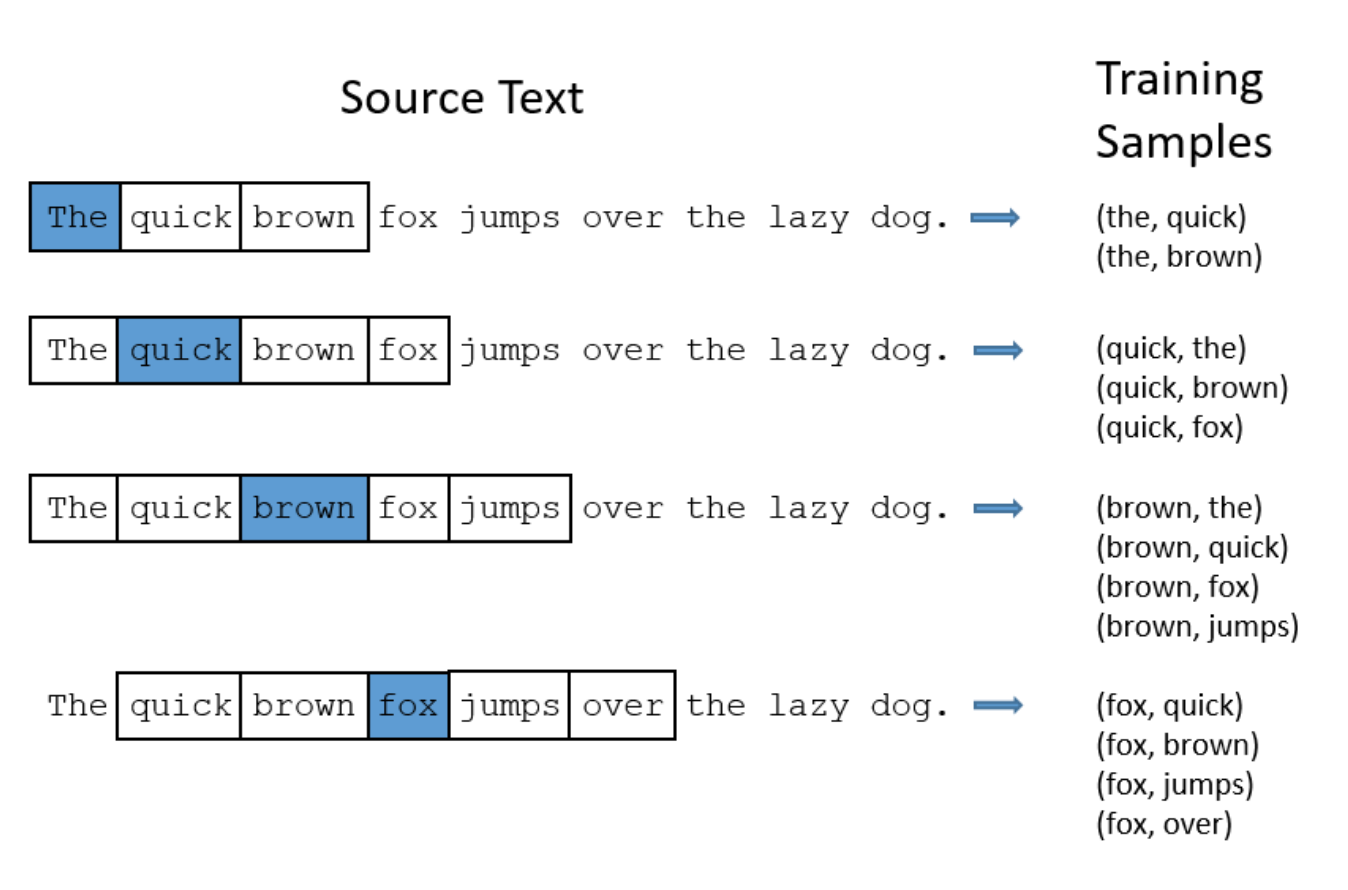
\includegraphics[width=0.5\textwidth]{figures/wordpairs}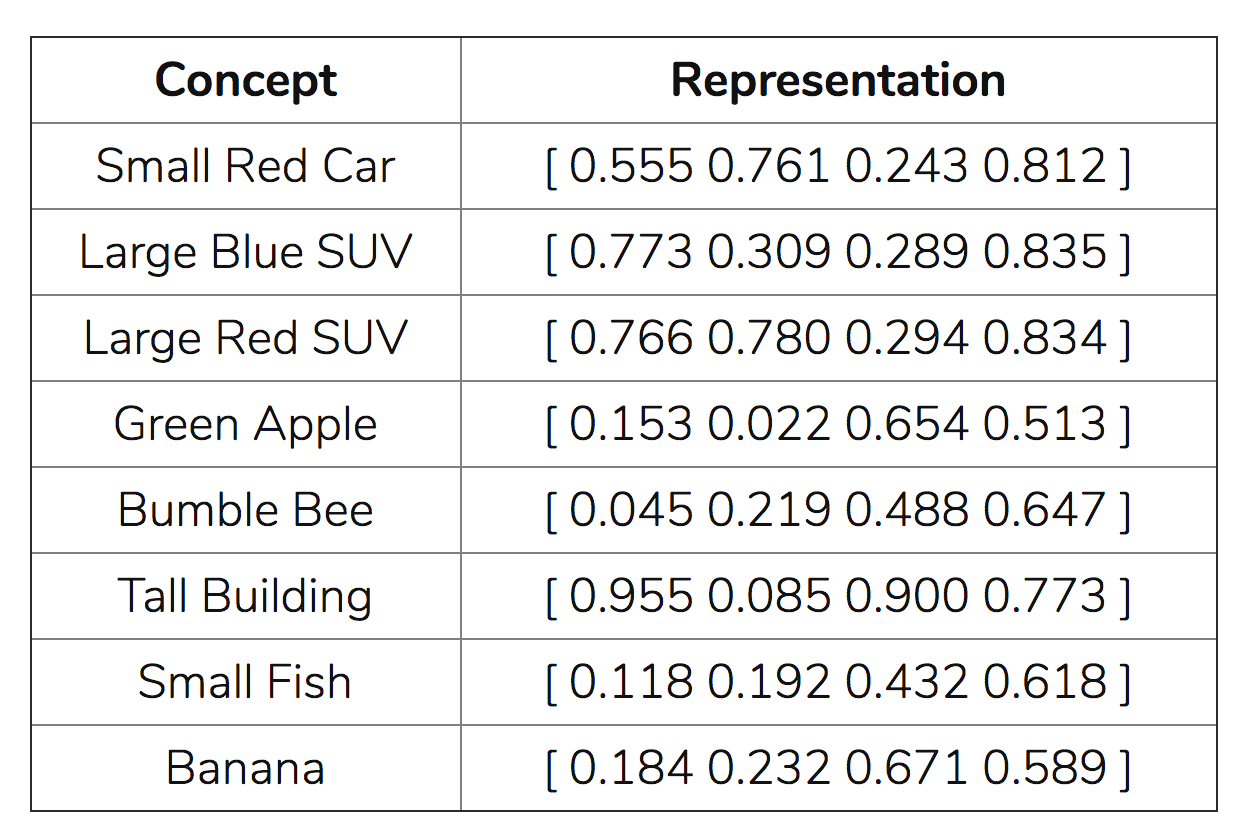
\includegraphics[width=0.5\textwidth]{figures/wordvecs}
%
%% \tiny{Pic from: \url{http://mccormickml.com/2016/04/19/word2vec-tutorial-the-skip-gram-model/}}
%% \end{frame}
%
%% \begin{frame}{The SkipGram model as LM}
%
%% Predicts the probability that some word occurs in {\it some} context (flexible! compared to n-gram)
%
%% \vspace{0.5cm}
%
%%     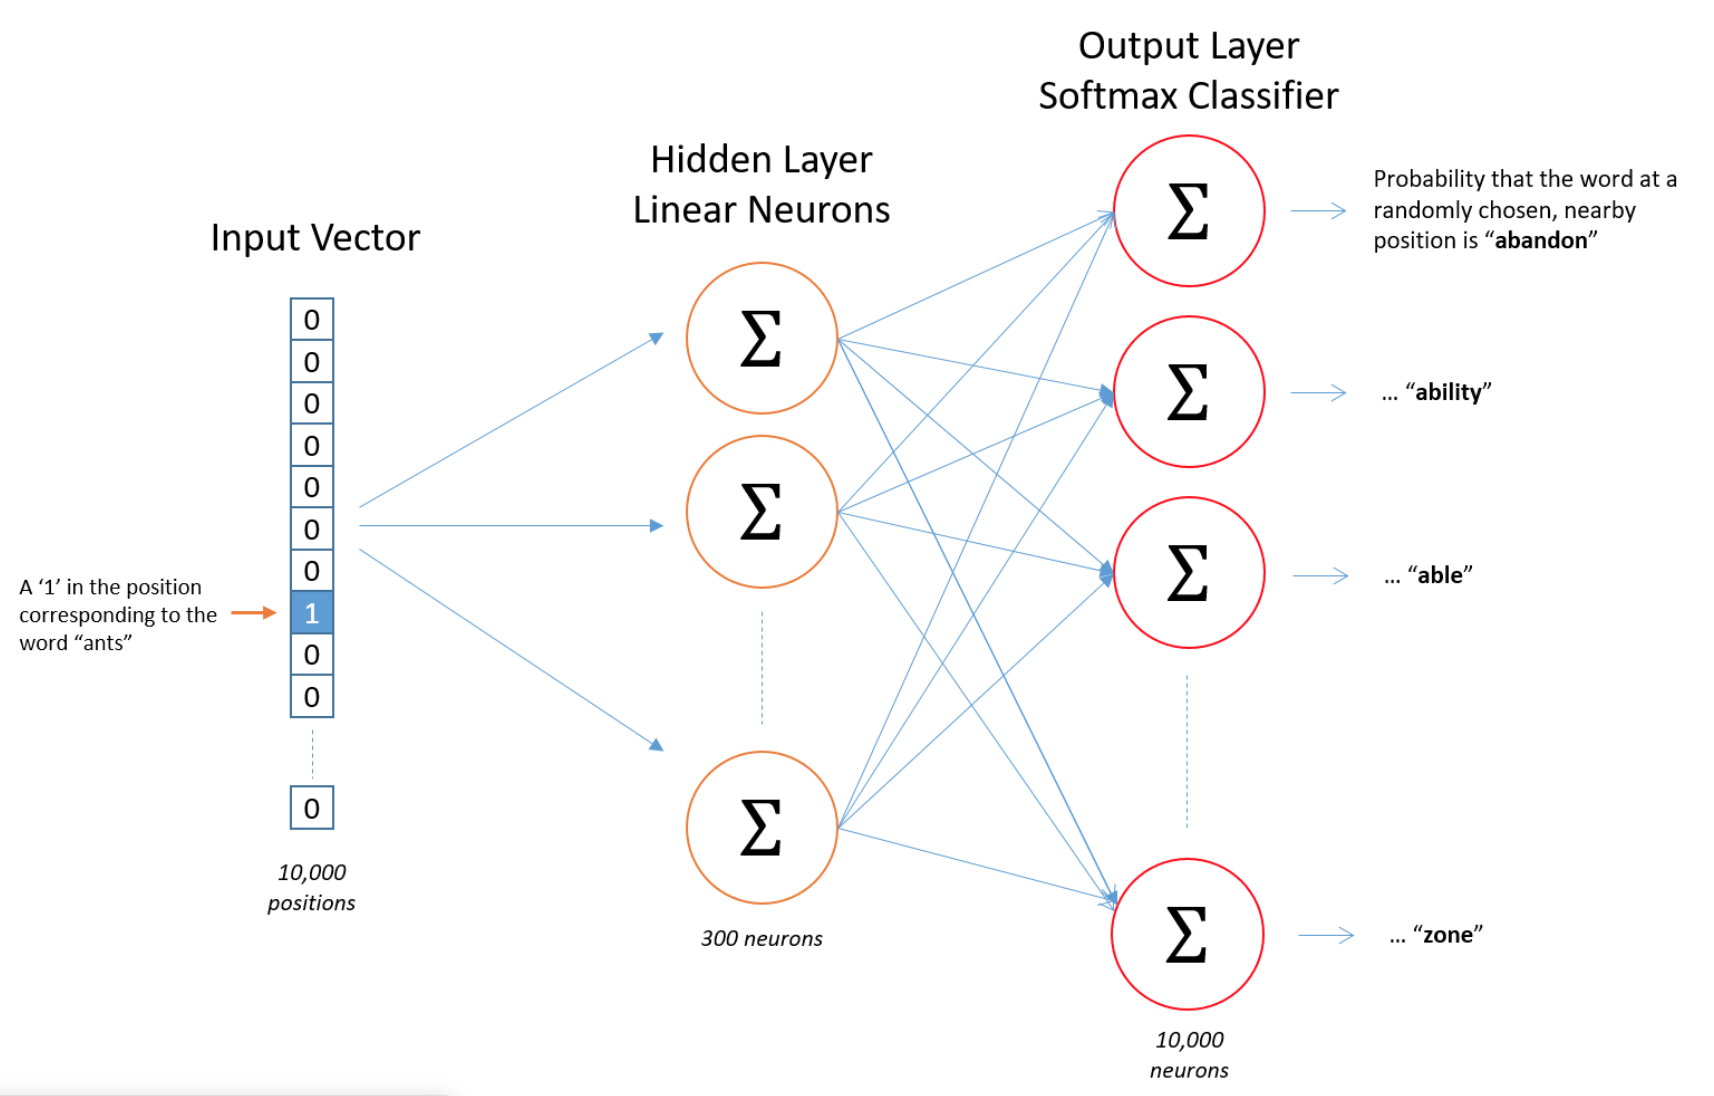
\includegraphics[width=0.8\textwidth]{figures/skipgram1} 
%    
%%     \tiny{Pic from: \url{http://mccormickml.com/2016/04/19/word2vec-tutorial-the-skip-gram-model/}}
%% \end{frame}
%
%% \begin{frame}{Exercise: Neural LMs vs. unsmoothed N-grams}
%% 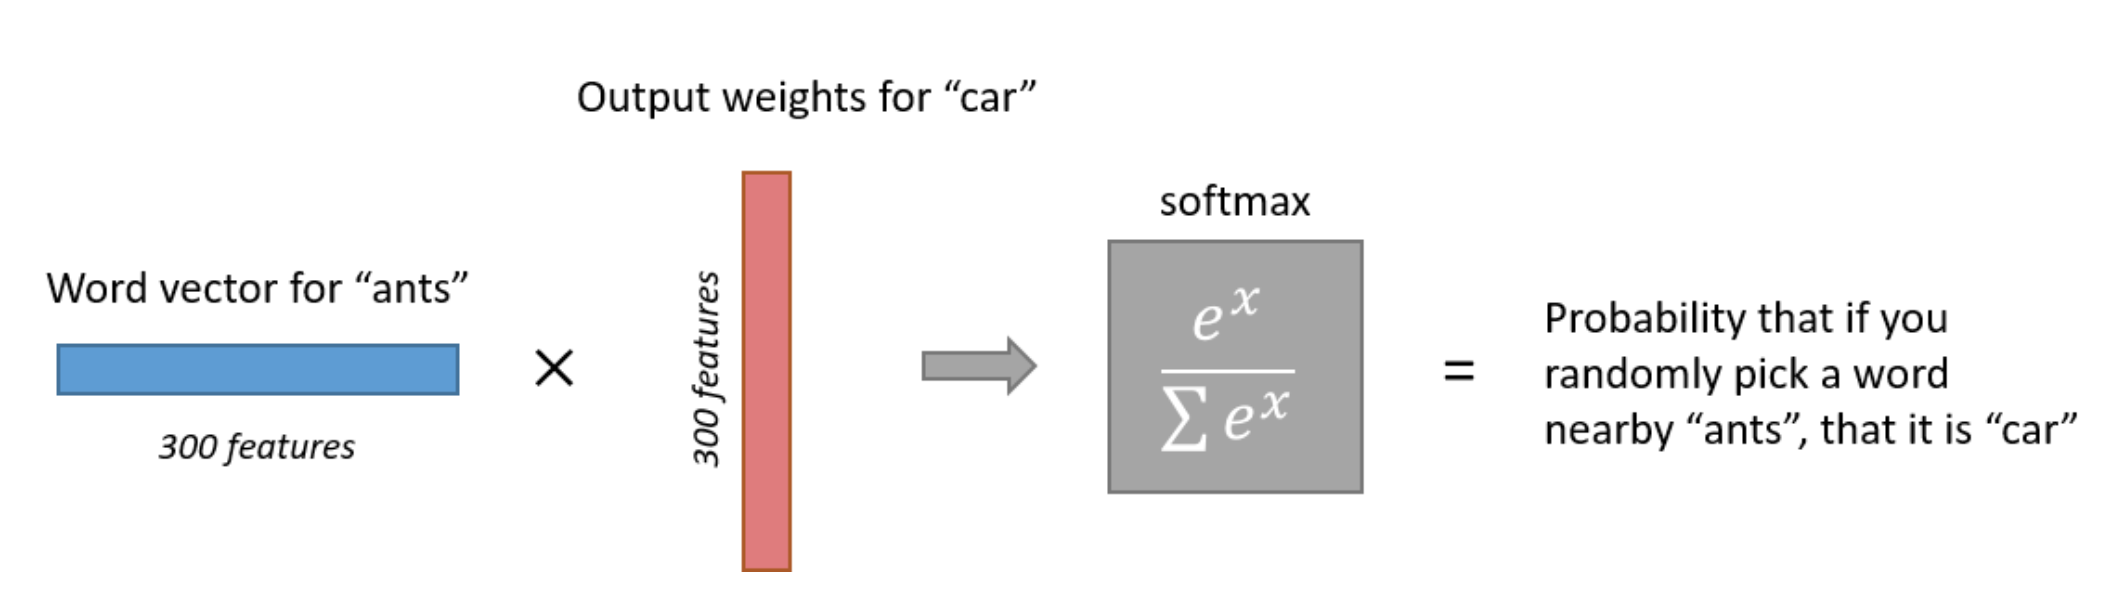
\includegraphics[width=0.9\textwidth]{figures/vector-multiplication}
%    
%%     \begin{itemize}
%%     \item N-gram models store probabilities that a word {\bf follows} a specific sequence of words
%%     \pause
%%         \item The input to the pre-trained neural LM is a word (vector), the output is the probability for each word in vocabulary of how likely it is to be in the input word's {\bf context window}
%%         %\item Suppose you have a corpus where each occurrence of the word {\it York} is preceded by {\it New}. You trained (1) an n-gram model and (2) a neural model on this corpus
%%         %\item What probability will n-gram model assign to {\York} following {\it New}?
%%         %\item Will the neural model assign the same probability?
%%         \pause
%%         \item Now, please fill out a poll: \url{https://pollev.com/olgazamaraev657}
%%         \pause
%%         \item Answer: a neural model will not give {\it York} a 100\% probability because we might want to pick another word from {\it New}'s context window
%%         \begin{itemize}
%%         \pause
%%             \item ...or more generally, another ``similar'' word
%%         \end{itemize}
%%     \end{itemize}
%    
%
%% \tiny{Pic from: \url{http://mccormickml.com/2016/04/19/word2vec-tutorial-the-skip-gram-model/}}
%% \end{frame}
%
%
%% \begin{frame}{Neural language models and word embeddings}
%
%    
%%     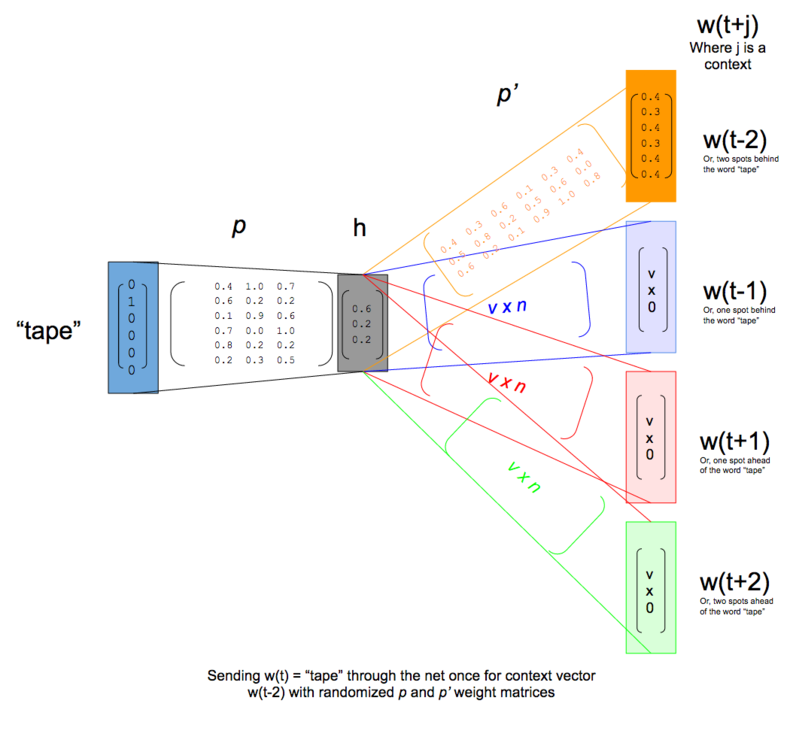
\includegraphics[height=0.9\textheight]{figures/skip-gram} 
%    
%
%%     {\tiny Figure from https://www.districtdatalabs.com/blog/}
%% \end{frame}
%
%
%
%% \subsection{Additional exercise: XOR}
%% \begin{frame}{Additional exercise: Why neural nets?}
%% \begin{itemize}
%%     \item A {\it neuron}:
%%     \begin{itemize}
%%         \item Input: vector
%%         \item Output: a single value
%%     \end{itemize}
%%     \item A {\it neural net}:
%%     \begin{itemize}
%%         \item Multiple computation units (neurons) combined
%%         \item Each unit takes a set of values and returns one value
%%         \item E.g. a sum of weighted observations
%%         \item Outputs of multiple units can be treated again as a vector and passed to other units!
%%         \item {\bf A non-linear transformation is essential for any NN}
%%     \end{itemize}
%% \end{itemize}
%% \end{frame}
%
%% \begin{frame}{Non-linearity and XOR: A case for neural nets}
%%     \begin{itemize}
%%         \item A non-linear transformation is essential for NN
%%         \item Why is it so useful?
%%     \end{itemize}
%% \end{frame}
%
%% \begin{frame}{Non-linearity}
%%     \begin{itemize}
%%         \item A non-linear transformation is essential for NN
%%         \item Why is it so useful?
%%         \begin{itemize}
%%             \item Data is often {\it linearly inseparable} unless we assume very high number of dimensions (which is often problematic)
%%         \end{itemize}
%%     \end{itemize}
%    
%%     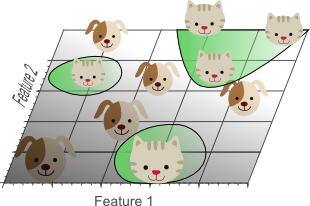
\includegraphics[height=0.5\textheight]{figures/overfitting}
%%     \tiny{picture from \url{http://www.visiondummy.com/2014/04/curse-dimensionality-affect-classification/}}
%% \end{frame}
%
%% \begin{frame}{XOR logical operator: A case for neural nets}
%%     \begin{itemize}
%%         \item {\bf A XOR B} is true only in two cases:
%%         \begin{itemize}
%%             \item A is True, B is False
%%             \item A is False, B is True
%%         \end{itemize}
%%     \end{itemize}
%    
%%     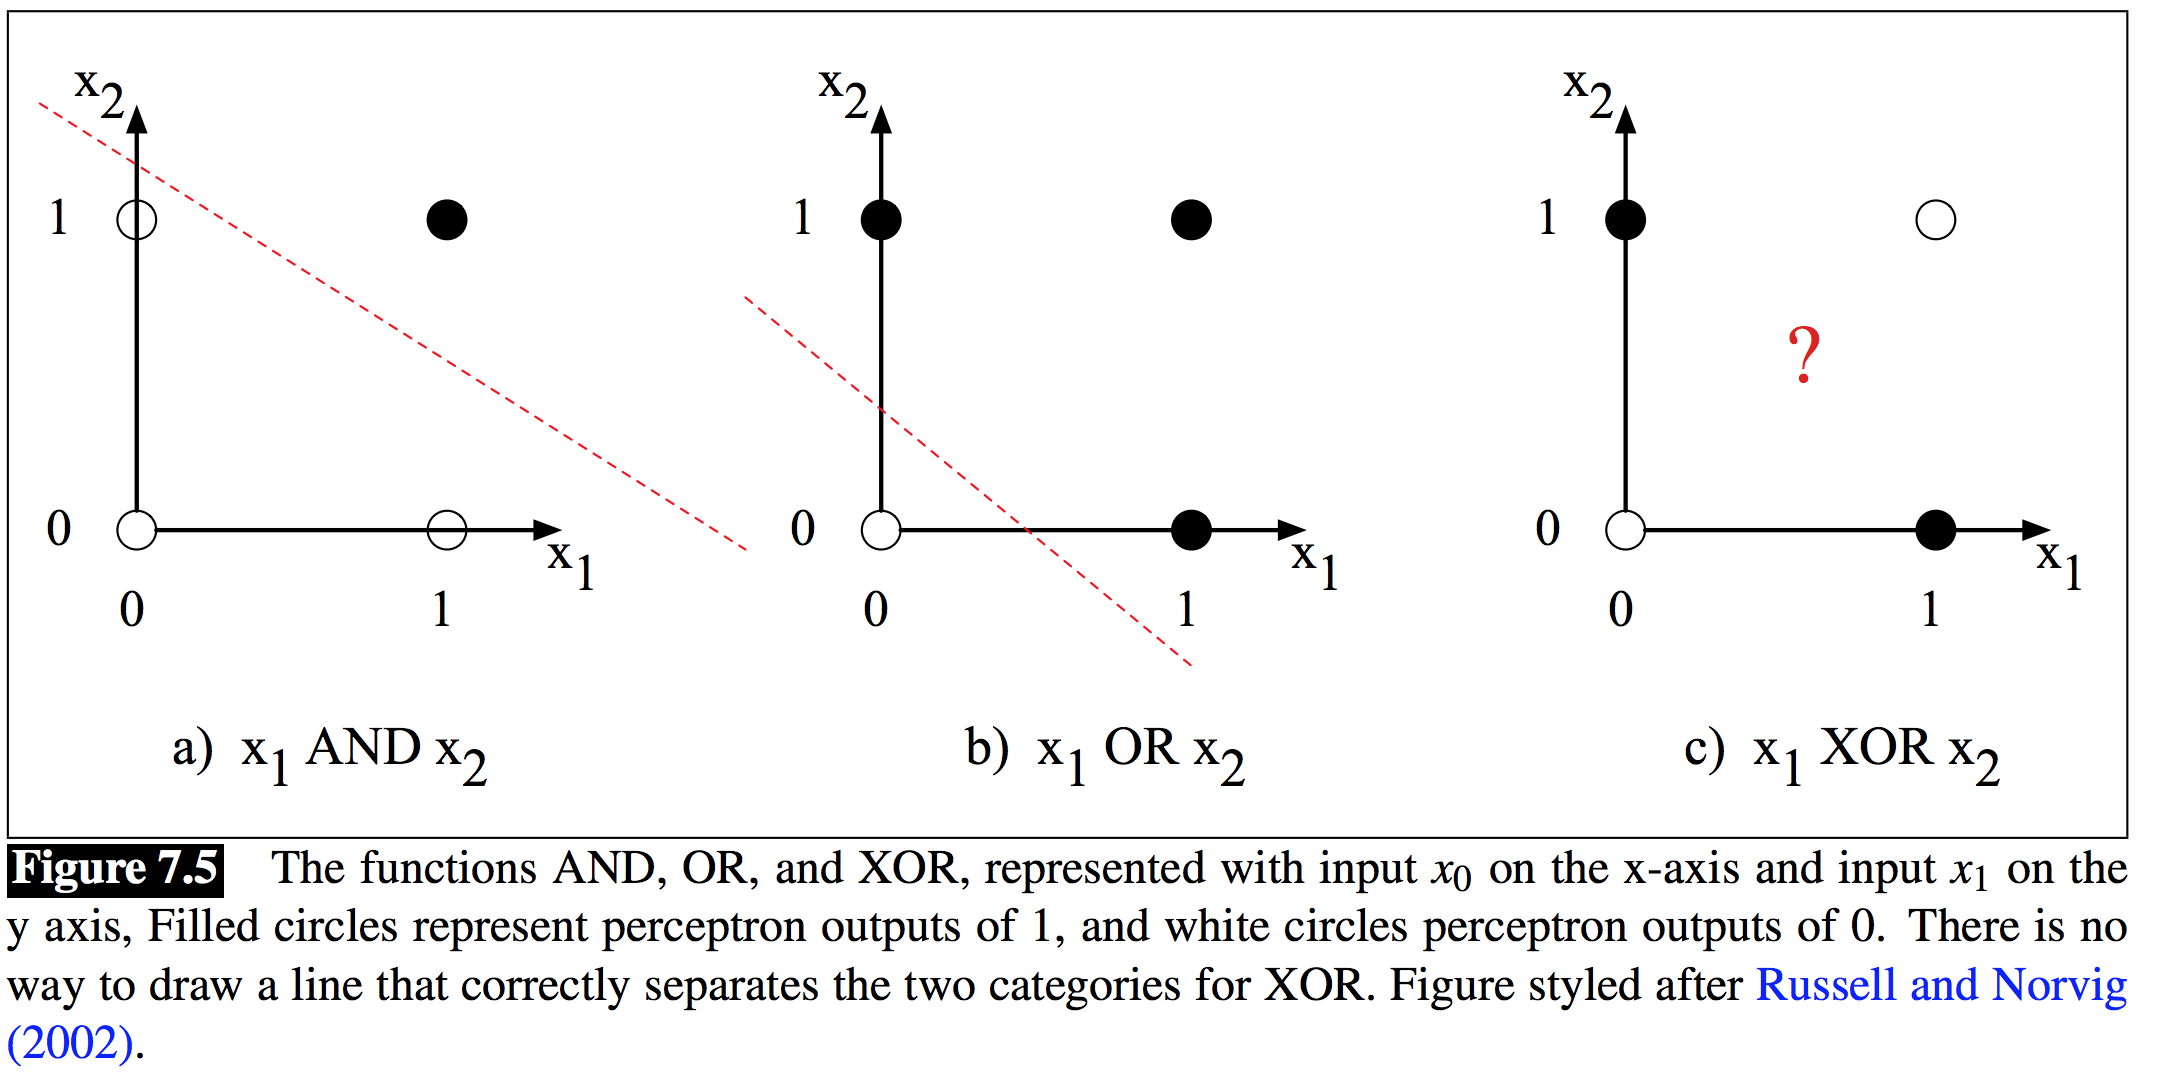
\includegraphics[width=\textwidth]{figures/xor1} 
%    
%%     {\tiny Figure from Jurafsky\&Martin, forthcoming}
%% \end{frame}
%
%% \begin{frame}{XOR logical operator: A case for neural nets}
%% \begin{small} 
%% e.g.\ x1 = 1, x2=1. What comes into h (and then y)? What comes out of h ( h computes the weighted sum of x1 and x2)? NB: each unit is a ReLU, so negative values will be mapped to 0.
%% \end{small}
%
%% 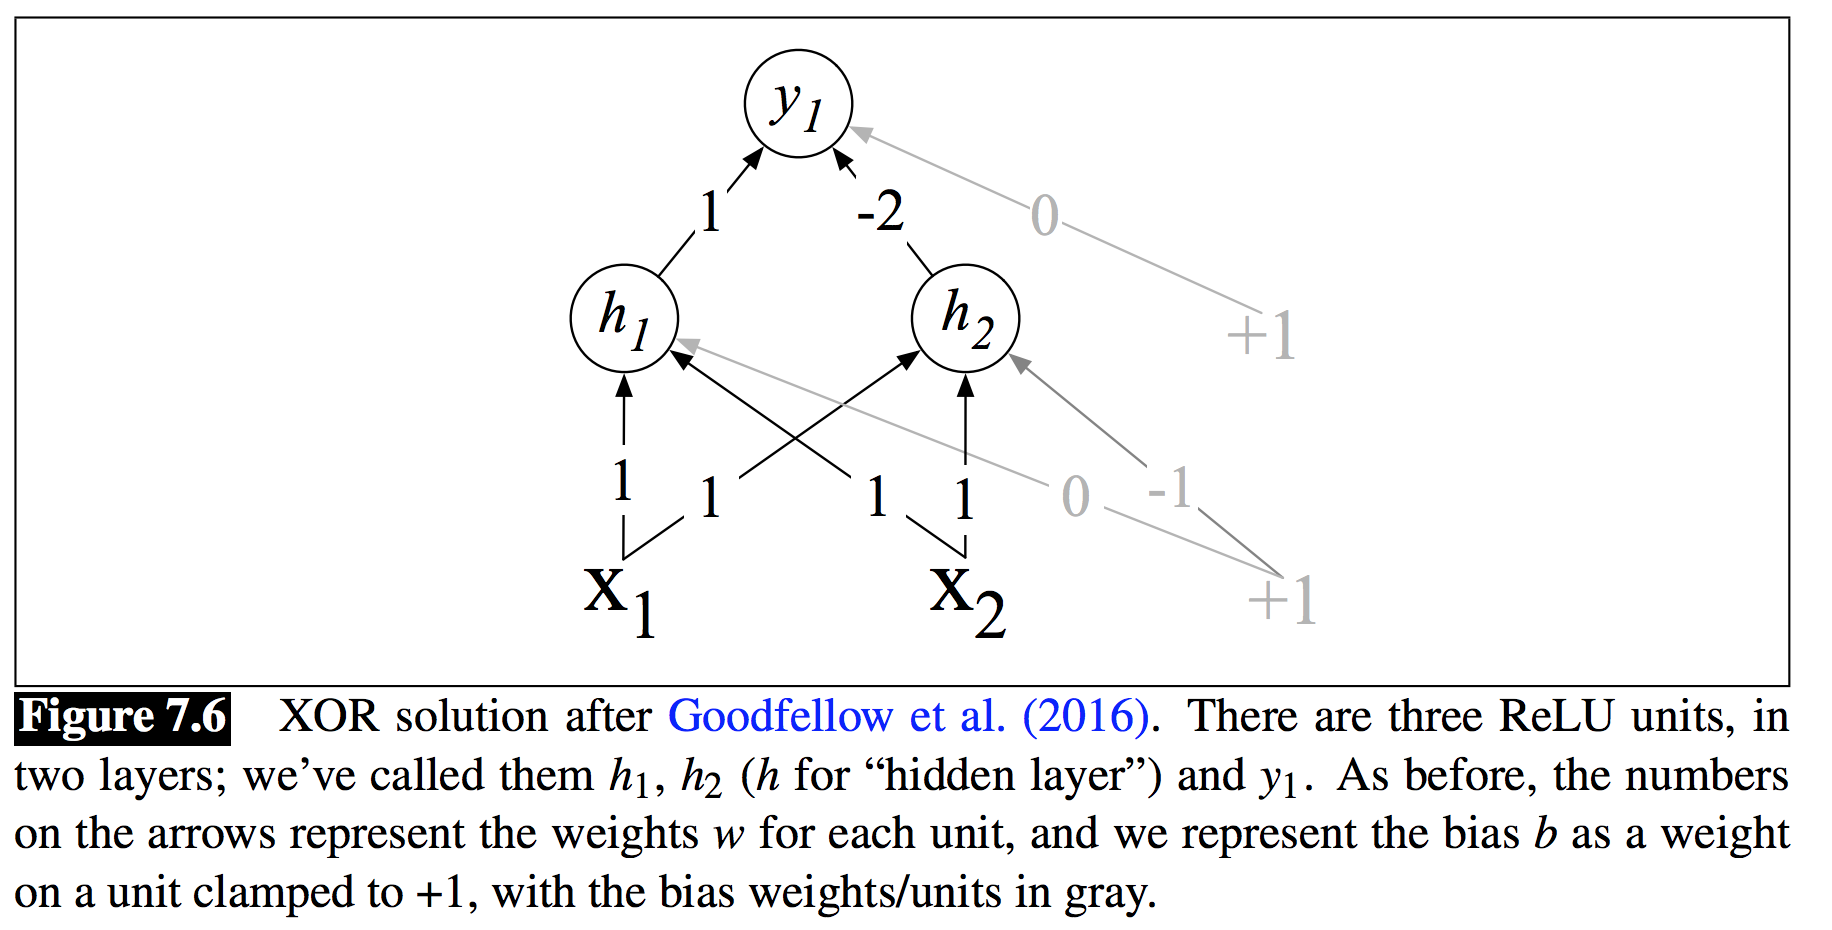
\includegraphics[width=\textwidth]{figures/xor-neural} 
%    
%%     {\tiny Figure from Jurafsky\&Martin, forthcoming}
%    
%% \end{frame}
%
%% \begin{frame}{XOR logical operator: A case for neural nets}
%
%
%% 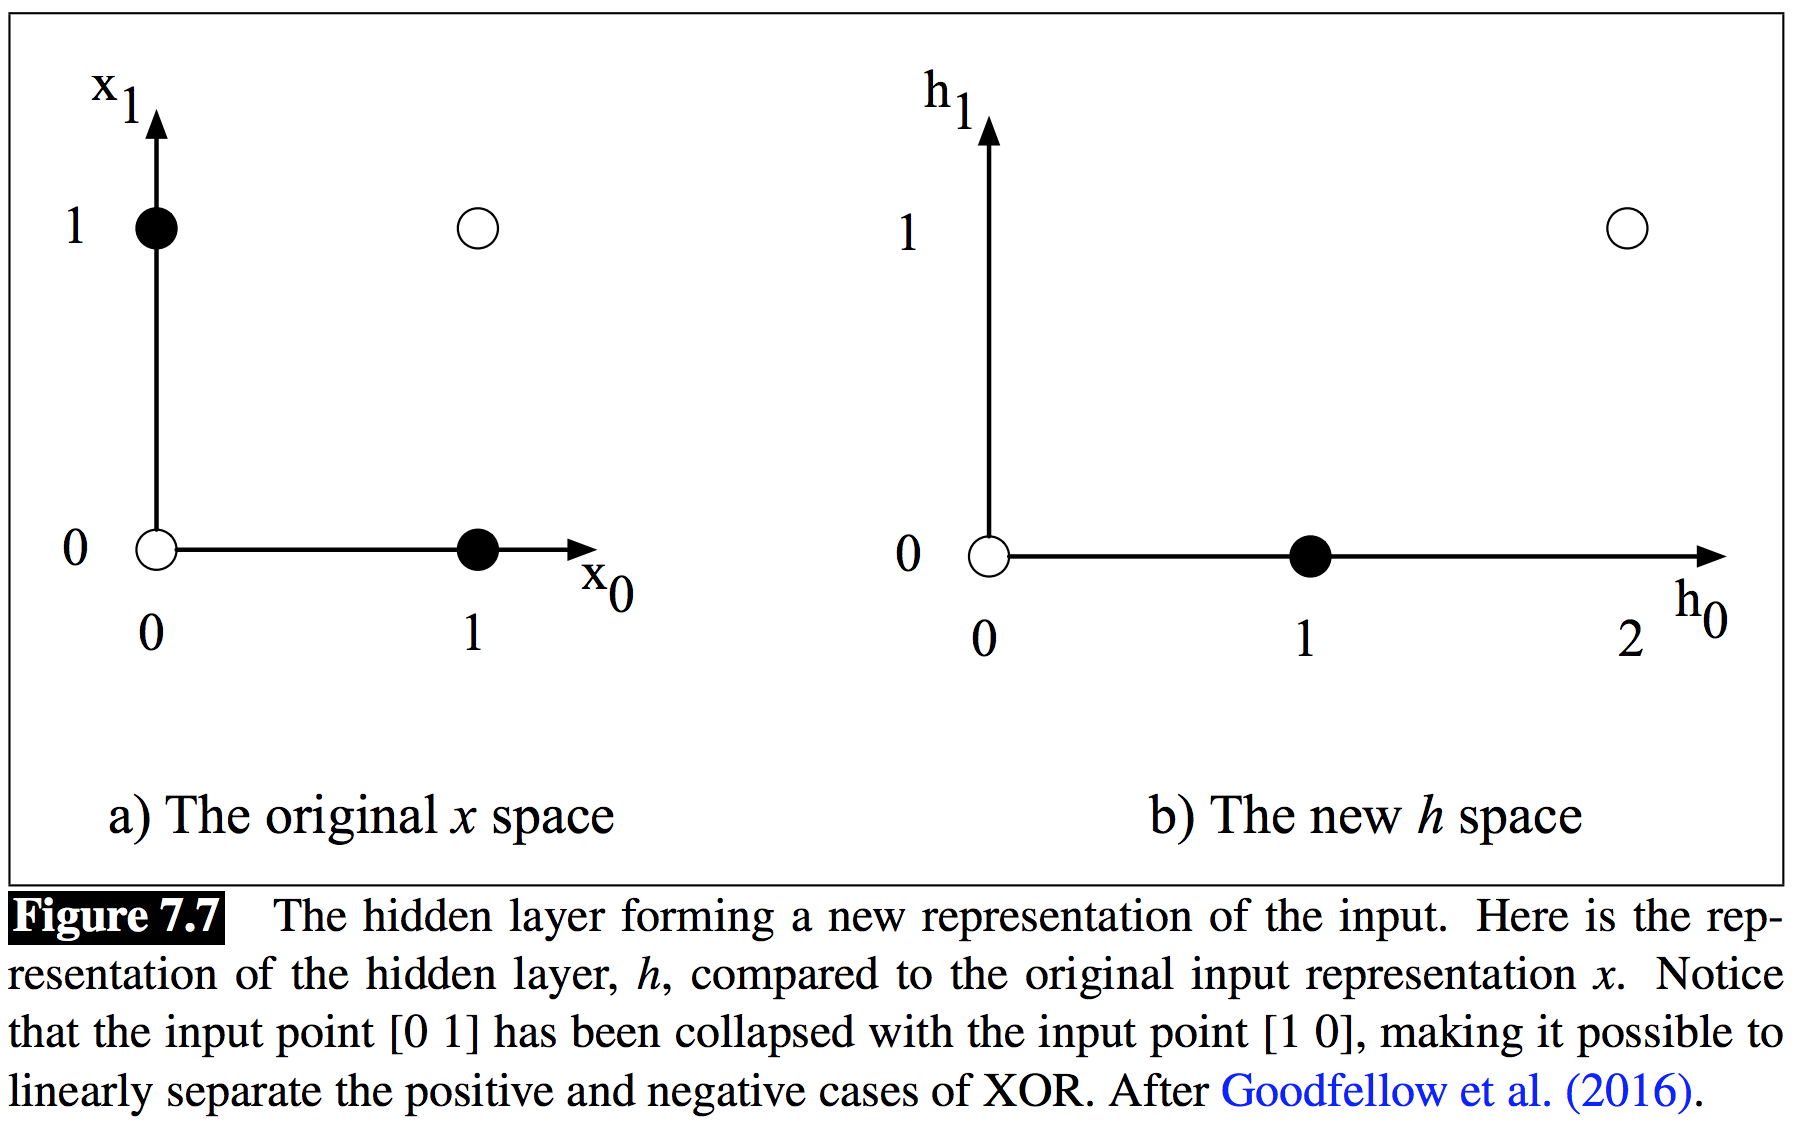
\includegraphics[width=\textwidth]{figures/xor-reduced} 
%    
%%     {\tiny Figure from Jurafsky\&Martin, forthcoming}
%    
%% \end{frame}
%
%
%%\section{Evaluation}
%% \begin{frame}
%% \frametitle{Evaluating N-gram models}
%% \begin{itemize}
%% \item What kinds of extrinsic evaluation are possible?
%% \item What kinds of intrinsic evaluation are possible?
%% \item What different kinds of models could you compare?
%% \end{itemize}
%% \end{frame}
%
%% \section{Evaluation}
%% \begin{frame}
%% \frametitle{Evaluating language models}
%% \begin{itemize}
%% \item What kinds of extrinsic evaluation are possible?
%% \begin{itemize}
%% \item ASR, MT, text generation
%% \end{itemize}
%% \item What kinds of intrinsic evaluation are possible?
%% \begin{itemize}
%% \item Perplexity: Given an n-gram model trained on some training set, how well does it predict the test set? (i.e., what probability does it assign to the test set?)
%% \end{itemize}
%% \item What different kinds of models could you compare?
%% \begin{itemize}
%% \item Different: training data, smoothing/back-off techniques, higher-level tokens
%% \end{itemize}
%% \end{itemize}
%% \end{frame}
%
%% \begin{frame}
%% \frametitle{Perplexity (intrinsic evaluation)}
%% \begin{itemize}
%% \item Which model assigns the {\bf highest probability} to the test set?
%% \item {\it Perplexity (PP)} is the inverse probability normalized by word count 
%% \begin{itemize}
%% \item We use perplexity and not probability because of a connection to information theory
%% \end{itemize}
%% \item E.g. for a test set $W = w_1w_2w_3...w_N$
%% \end{itemize}
%
%% $PP(W) = P(w_1w_2w_3...w_N)^{\frac{-1}{N}} = (\prod_{i=1}^N{P(w_i\vert w_1...w_{i-1})})^{\frac{-1}{N}}$
%
%% \vspace{0.5cm}
%
%% $\approx (\prod_{i=1}^N{P(w_i\vert w_{i-1})})^{\frac{-1}{N}}$
%
%% \end{frame}
%
%% \begin{frame}
%% \frametitle{Perplexity}
%
%% \begin{itemize}
%% \item Perplexity can bee seen as an average {\it branching factor} of a language
%% \item e.g. consider a language of digits where each digit has a probability of 0.1 of following another digit
%% \end{itemize}
%
%% $PP(W) = P(w_1w_2...w_N )^{-\frac{1}{N}}=$
%% %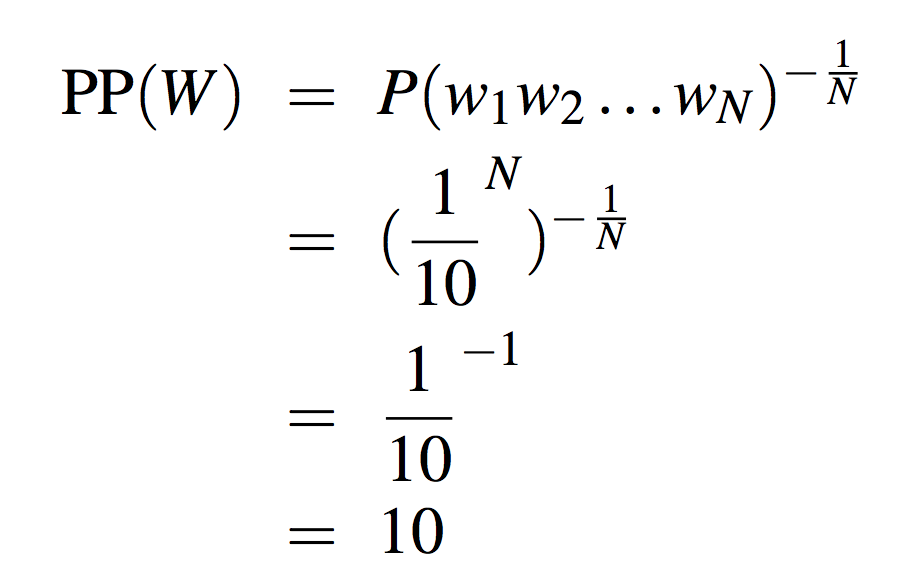
\includegraphics[height=0.5\textheight]{figures/ppl}
%
%% \vspace{4cm}
%
%% Is this high perplexity?
%
%% \end{frame}
%
%
%% \begin{frame}
%% \frametitle{Perplexity}
%
%% \begin{itemize}
%% \item Perplexity can bee seen as an average {\it branching factor} of a language
%% \item e.g. consider a language of digits where each digit has a probability of 0.1 of following another digit
%% \end{itemize}
%
%% 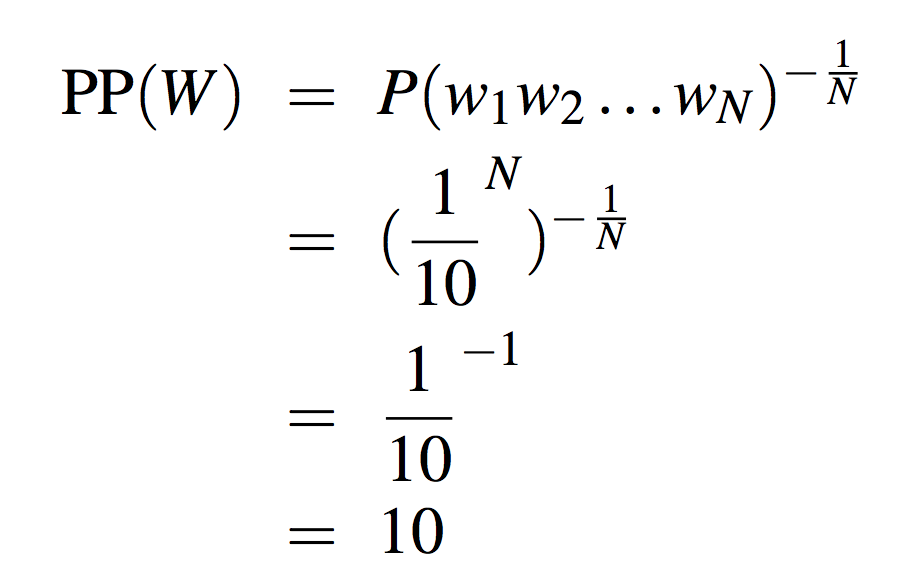
\includegraphics[height=0.5\textheight]{figures/ppl}
%
%% Is this high perplexity?
%
%% \end{frame}
%
%\begin{frame}{SkipGram training (simplified)}
%    
%    \begin{itemize}
%        \item Keep changing the p and p' matrices until the output probabilities are similar to the training corpus
%        \item In the training corpus, count how many times a word occurs in the context of some other word and compute probabilities:
%    \end{itemize}
%    
%    \vspace{0.2cm}
%    
%    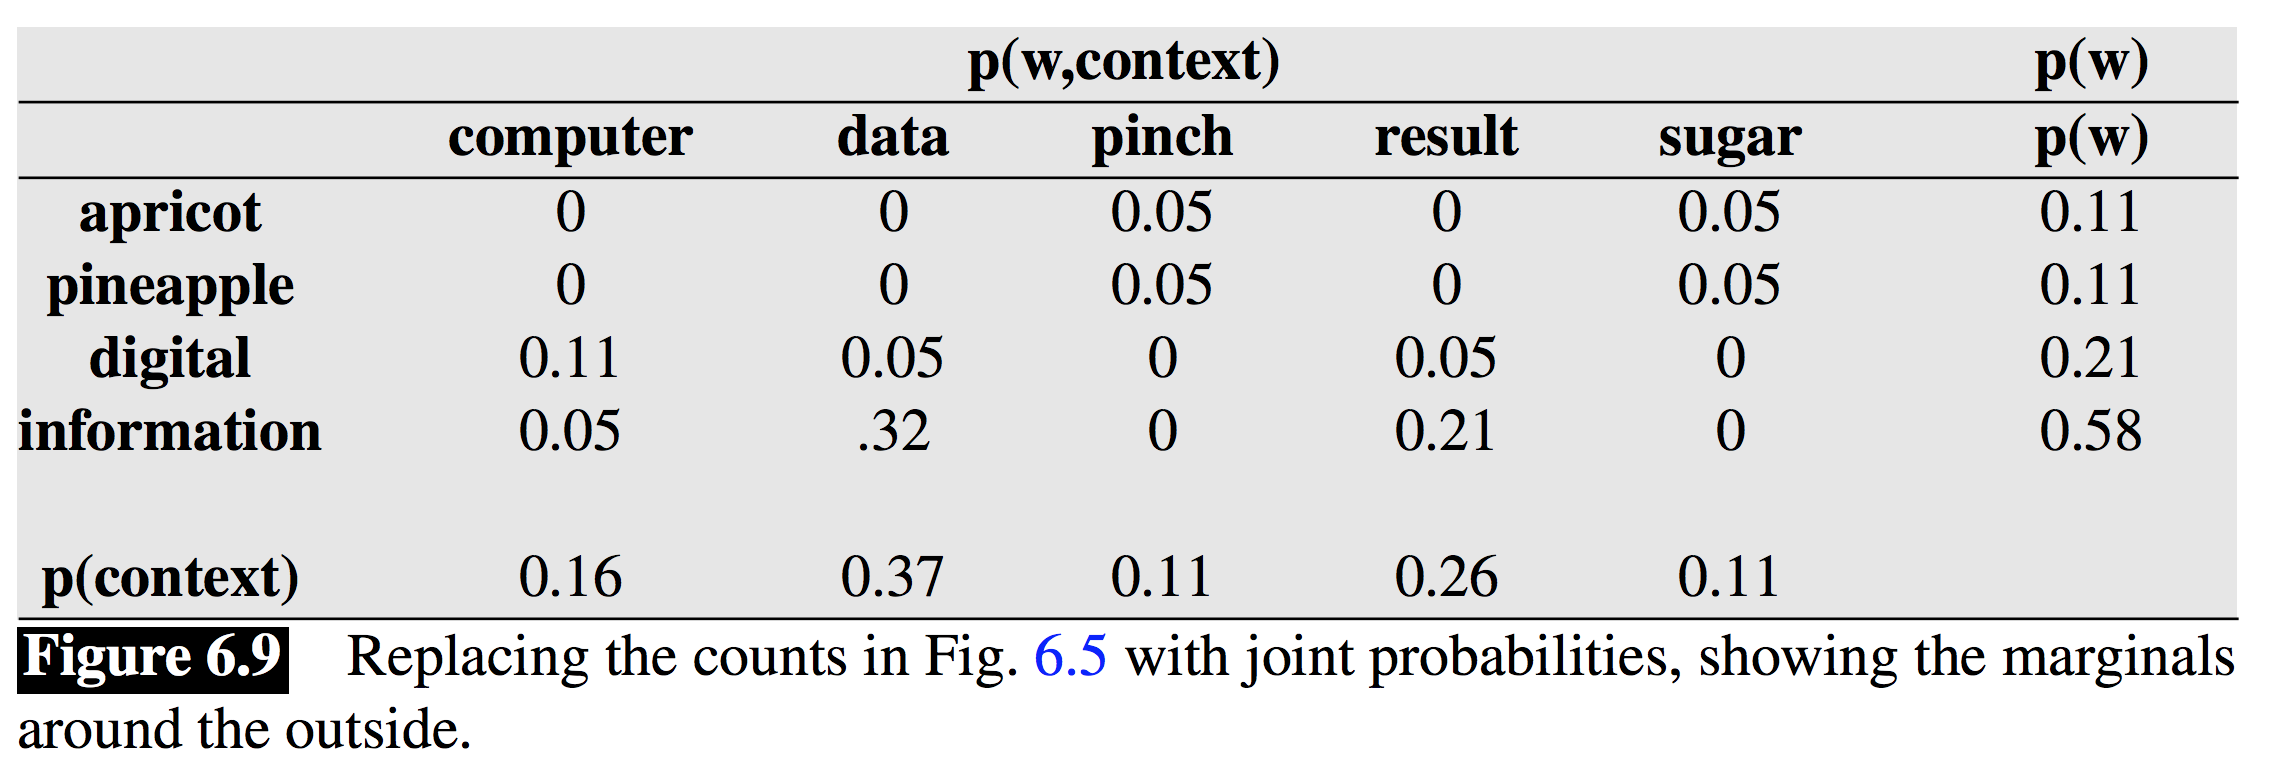
\includegraphics[width=\textwidth]{figures/sparse-vec-prob}
%    
%    \vspace{0.2cm}
%    
%    \begin{itemize}
%        \item Observe that we train to output accurate {\it probabilities} but it is the same as to train words that occur in similar contexts to have {\it similar vector representations}
%    \end{itemize}
%    
%\end{frame}
%
%% \begin{frame}{What are vector space models trying to accomplish?}
%
%% \begin{itemize}
%%     \item Historically, Latent Semantic Analysis (Landauer \& Dumais 1997):
%%     \begin{itemize}
%%         \item The goal is to explain how knowledge is acquired
%%         \item Including: how do people acquire language so quickly?
%%     \end{itemize}
%%     \item In modern NLP, these representations are seen mostly as convenient/leading to score improvements
%%     \item Neural networks are used instead of LSA
%% \end{itemize}
%% \end{frame}
%
%% \begin{frame}{Words as dense vectors}
%
%% \begin{itemize}
%%     \item decide on a small number of dimensions
%%     \item want similar words to have similar vectors
%%     \item like in the example below:
%%     \begin{itemize}
%%         \item  (But where would these numbers come from?)
%%     \end{itemize}
%% \end{itemize}
%
%
%
%% \vspace{0.5cm}
%
%% \begin{center}
%%       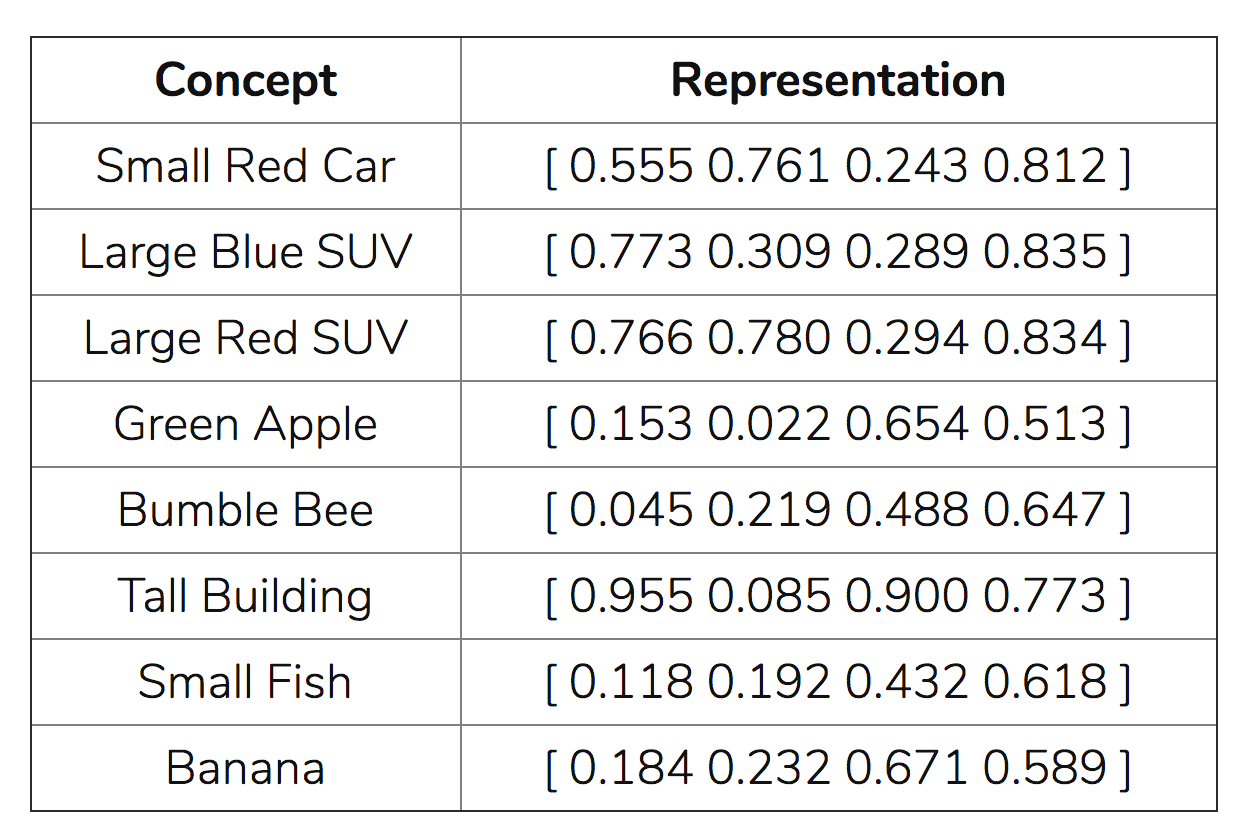
\includegraphics[height=0.5\textheight]{figures/wordvecs}
%% \end{center}
%
%%     \vspace{0.2cm}
%    
%%     \tiny{figure from: \url{https://www.districtdatalabs.com/nlp-research-lab-part-1-distributed-representations/}}
%    
%    
%% \end{frame}
%
%\begin{frame}{Distributional semantics}
%We used a huge VxV matrix for training but we do not generally need huge dimensions to represent similar words as similar vectors: 
%
%\vspace{0.2cm}
%
%    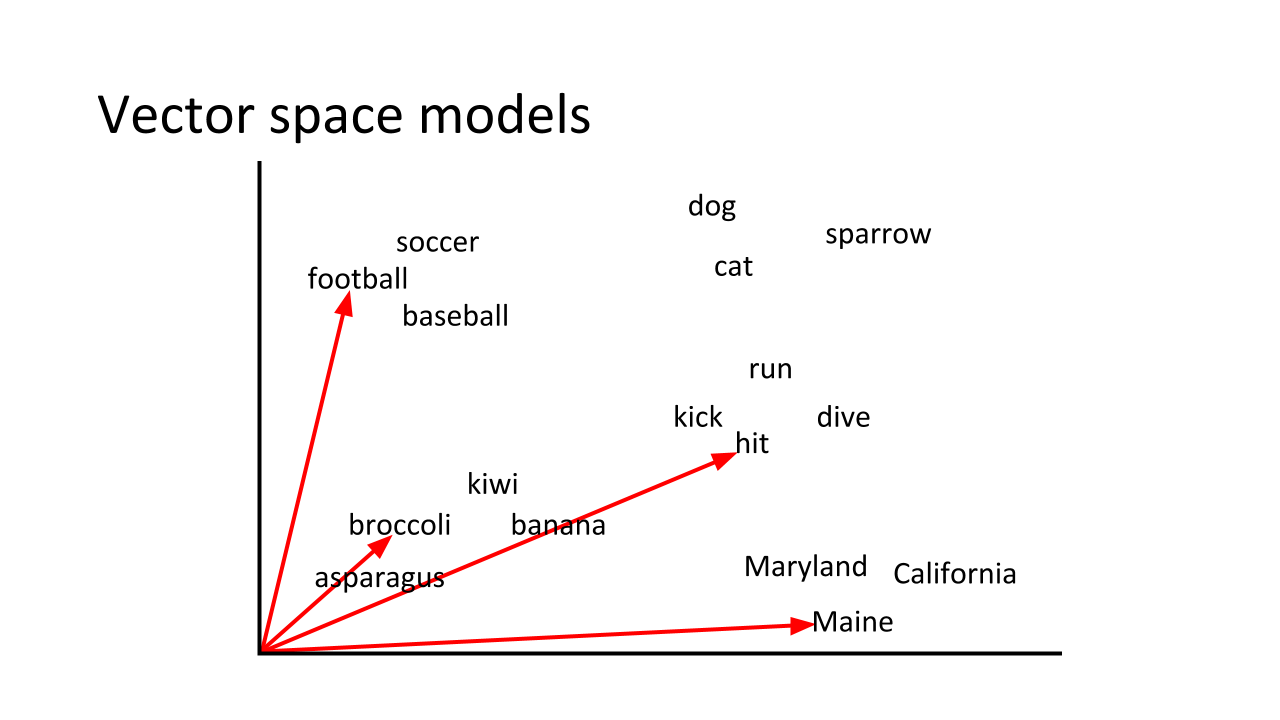
\includegraphics[width=\textwidth]{figures/vector-space.png}
%    
%    \vspace{0.1cm}
%    
%    NB: We define vector {\it similarity} in terms the {\bf direction} (recall also {\bf cosine}) -- length and origin do not matter
%    
%    {\tiny Figure from Allyson Ettinger's tutorial SCiL 2019}
%\end{frame}
%
%\begin{frame}{The SkipGram model: Dense vectors}
%
%\begin{minipage}{0.6\textwidth}
%    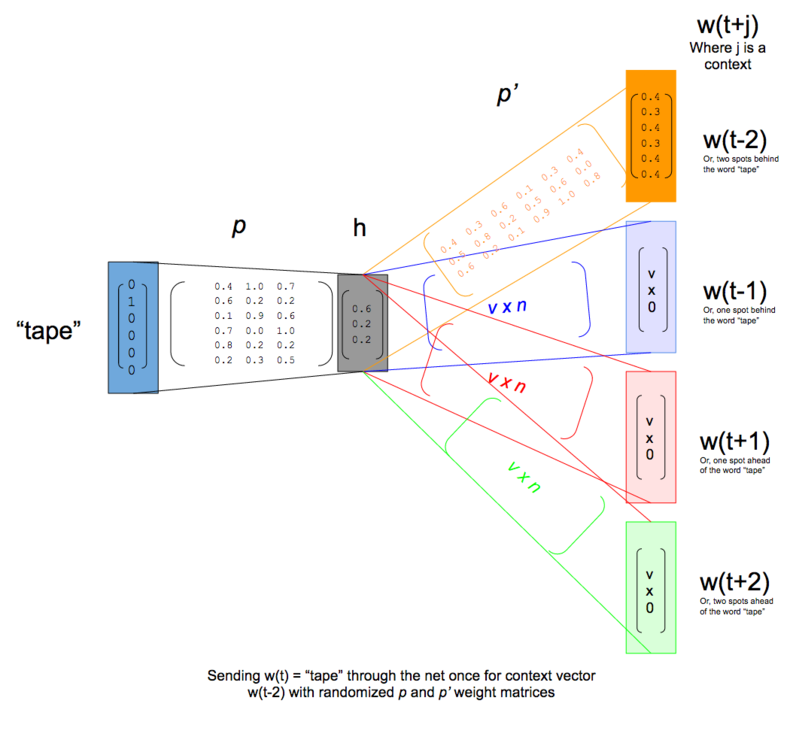
\includegraphics[width=\textwidth]{figures/skip-gram} 
%\end{minipage}
%\begin{minipage}{0.3\textwidth}
%\begin{itemize}
%    %\item computation is the {\it dot product}: $p \cdot h$, $h \cdot p'$
%    %\item cosine is related to dot product
%    \item vectors in p will end up similar for similar words
%    \item ...but p is not a VxV matrix, it is Vxd where d is small
%\end{itemize}
%\end{minipage}
%    
%    \tiny{Pic from: \url{https://medium.com/district-data-labs/forward-propagation-building-a-skip-gram-net-from-the-ground-up-9578814b221}}
%\end{frame}
%
%\begin{frame}{(Simplified) neural models architecture}
%
%% \begin{columns}[T] % align columns
%% \begin{column}{.20\textwidth}
%
%% \end{column}%
%% \end{columns}
%\begin{small}
%\begin{itemize}
%    \item The SkipGram model (Mikolov et al)
%    \item Outputs probabilities of words occurring in contexts...
%    \item Produces useful dense word vectors
%\end{itemize}
%
%\end{small}
%    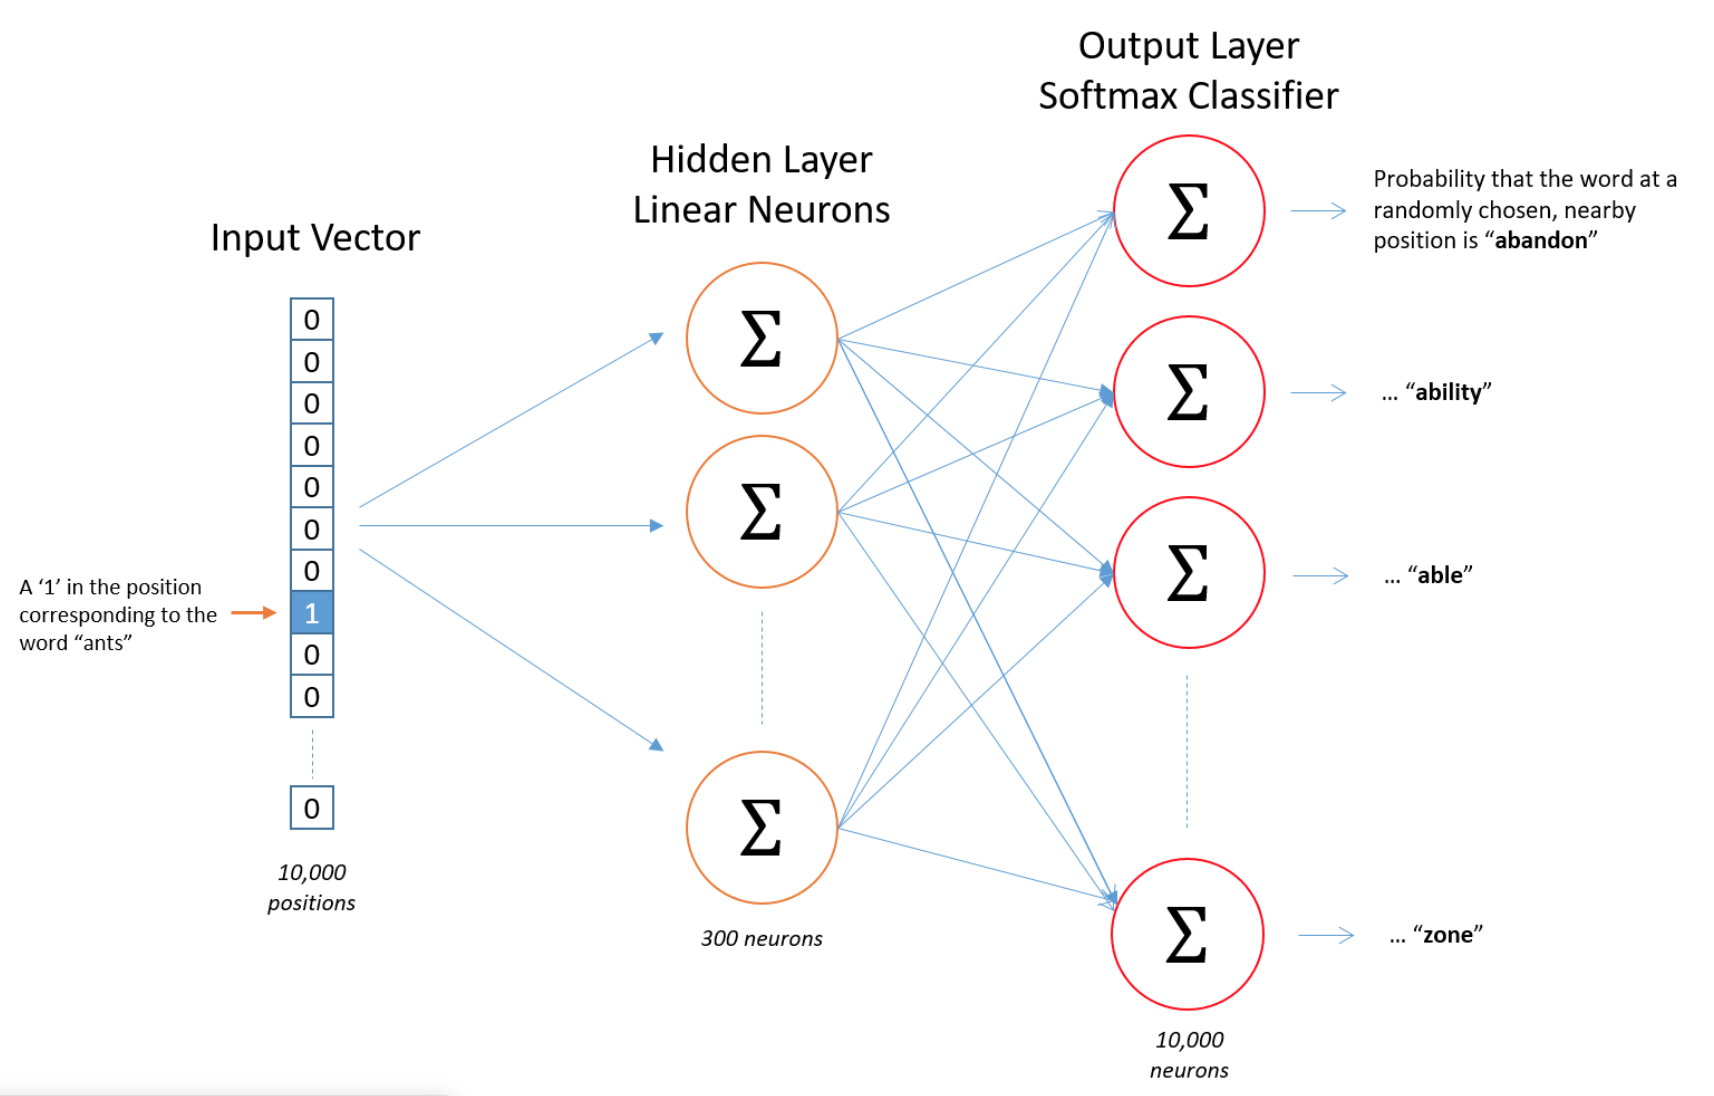
\includegraphics[width=0.9\textwidth]{figures/skipgram1}
%    
%    \tiny{Pic from: \url{http://mccormickml.com/2016/04/19/word2vec-tutorial-the-skip-gram-model/}}
%\end{frame}
%
%\begin{frame}{Word embeddings are useful for many NLP tasks}
%
%    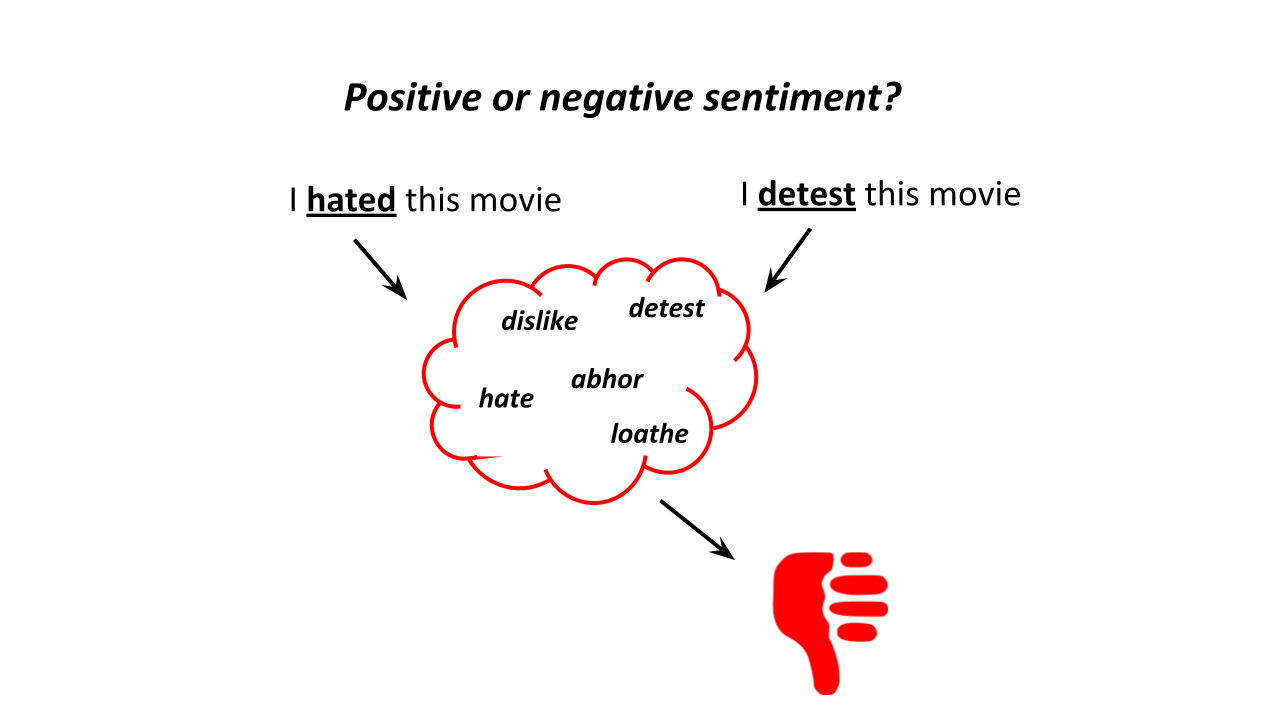
\includegraphics[width=0.9\textwidth]{figures/sentiment.png}
%    
%    \vspace{1.5cm}
%    
%    {\tiny Figure from Allyson Ettinger's tutorial at SCiL 2019}
%\end{frame}
%
%\begin{frame}{Bias in word embeddings (Bolukbasi et al. 2016)}
%Words are similar if their vectors are close to each other in the
%vector space:
%
%\begin{itemize}
%    \item Paris - France + Italy = Rome (fine)
%    \item king - man + woman = queen (ok)
%    \item man - programmer + woman = homemaker (ouch!)
%\end{itemize}
%
% 
% \begin{itemize}
% \item What is captured about words by that similarity?
% \begin{itemize}
%     \item the biases of the data that was used for training
% \end{itemize}
%     \item What is problematic about it?
%     \begin{itemize}
%     \pause
%         \item biases are amplified and reinforced through technology
%     \end{itemize}
% \end{itemize}
%\end{frame}


\section{Summary}
\begin{frame}
\frametitle{What you need to know}
\begin{itemize}
	\item What are N-grams?
	\item When are they useful?
	\item Simple (un-smoothed) N-grams
	\item Perplexity (relationship to probability and what for)
	\item (Next time) Unknown words, Smoothing, back-off, interpolation
\end{itemize}
\end{frame}



% \begin{frame}
% \frametitle{Will statistics take over everything?}

% aka Norvig vs.\ Chomsky debate

% My opinion:

% \begin{itemize}
% \item There is certainly truth to both sides
% \item The role of {\bf noise}:
% \begin{itemize}
% \item Chomsky: Noise does not matter
% \item Norvig: Noise exists
% \end{itemize}
% \item The role of {\bf elegance}:
% \begin{itemize}
% \item Chomsky: Elegance matters
% \item Norvig: But Chomsky's theory is far from elegant!
% \end{itemize}
% \item An ideal model would account for the actual rules of language yet won't pretend that noise does not exist
% \item ``If human understanding is not necessary, the role of the scientist might change forever'' (Kevin Gold)
% \item Isn't it already changing?..
% \end{itemize}
% \end{frame}

%\section{Lab preview}
%
%\begin{frame}{Lab prerequisites}
%\begin{itemize}
%    \item Basic python programming skills, especially understanding of lists and strings as lists
%    \item Patience with python versioning issues and packages installation
%    \item Time commitment: 5-10 hours of actual work, depending on your coding skills, and 10 hours of passive running time of neural training
%    %\item Machine learning concepts: loss, accuracy
%    \item (The write up portion assumes enough grading resources for the class size and aims at assessing a diverse range of learning outcomes)
%    %\item Perplexity as an evaluation metric for N-gram models (would be part of another, more in-depth lecture on N-grams)
%\end{itemize}
%    
%\end{frame}
%
%\begin{frame}{Lab goals}
%\begin{itemize}
%    \item Learn to use and adapt existing code for LMs
%    \item Informally ``evaluate'' LMs
%    \begin{itemize}
%    \item Evaluation is crucial in NLP
%    \item LMs can be evaluated {\it intrinsically}, e.g.\ using special {\it metrics}, and {\it extrinsically}, by looking at their performance on downstream tasks, e.g.\ text generation
%\end{itemize}
%\item Reflect on LMs applicability and limitations
%\item Reflect on what challenges human languages present to LMs
%\item Practice representing your work in a clear write up
%\end{itemize}
%
%
%\end{frame}
%
%\begin{frame}{Lab Exercise: N-gram and Neural language models}
%
%\begin{itemize}
%    \item In this lab, you will use a set of tools:
%    \begin{itemize}
%        \item to create some n-gram and neural language models
%        \item to use both types of models for text generation (informal ``extrinsic evaluation'')
%        \item you are also likely to experience some joys of python versioning and package installation, unless you have access to a pre-set up machine
%    \end{itemize}
%\end{itemize}
%
%\end{frame}
%
%% \begin{frame}{Lab Exercise, Part I: N-gram models}
%% (This lab was originally put together by Glenn Slayden)
%%     \begin{itemize}
%%     \item Train a a series of n-gram language models on the complete Sherlock Holmes stories file from the Project Gutenberg website using the instructions (and some historic software!):
%%     \begin{itemize}
%%         \item \url{http://courses.washington.edu/ling472/sp2018/hw/hw3/assignment3.html} (see Part II)
%%     \end{itemize}
%%     %\item Instead of the software mentioned in the lab, use python and NLTK model
%%     %\item Implement the function to compute perplexity yourself
%%     \item Evaluate how well the models model different texts, per the instructions on the website
%% \end{itemize}
%% \end{frame}
%
%\begin{frame}{Lab, Part I: N-gram models}
%Take the character-based n-gram model put together by Yoav Goldberg:
%
%    \begin{itemize}
%        \item {\tiny{\url{https://nbviewer.jupyter.org/gist/yoavg/d76121dfde2618422139?fbclid=IwAR0GEfBE3WWwXiTVmUKr0YsIZc6DAzSDqvZiMlKYPQajv4-As1vvqL0FAKk}}}
%        \item \footnotesize{Make sure you observe the behavior that the notebook is describing}
%        \item Change the model to be word-base (write new functions for training and generation; they can be very similar, you just need to make a connection between a string and a list in python)
%        \item Train a bigram, a trigram, and a quadrigram model using the Sherlock Holmes story ``His last bow'' (Project Gutenberg or course website).
%        \item Generate and save some text (1000 words) using bigrams, trigrams, quadrigrams
%        %\item In the write up, discuss any linguistic differences of the 3 outputs
%    \end{itemize}
%    
%\end{frame}
%
%\begin{frame}{Lab Exercise, Part II: Neural models}
%Based on Jason Brownlee's tutorial {\footnotesize \url{https://machinelearningmastery.com/how-to-develop-a-word-level-neural-language-model-in-keras/}}. 
%\begin{itemize}
%    \item Complete the tutorial using the same text ({\it His last bow}) as in the previous part 
%    \item Train 3 neural models: 1 epoch, 10 epochs, 100 epochs (allow for an overnight run if using your own non-GPU computer for the 100 epochs). {\bf Save} each in a file, be careful {\bf not to overwrite}. {\bf Record} the time it took to train each model
%    \item Build a 10-epoch model using the {\it entire} Sherlock Holmes collection (course website)
%    \item Generate and {\bf save} 1000 words using each of the 4 models 
%    \item Train a model in 100 epochs on Balzac's {\it La comédie humaine} and generate and {\bf save}  1000 words. 
%\end{itemize}
%\end{frame}
%    
%    \begin{frame}{Lab: Write up}
%    Your write up will have 8 concise sections, a section per question (2-4 pages total):
%    
%    \begin{itemize}
%        \item[1.] In a table, compare the time it took to train the neural models to n-gram. Discuss the reasons behind that.
%        \item[2.]  Discuss the differences between the text generated by the bigram, trigram, and 4-gram models
%        \item[3.] Discuss the differences between the text generated by the 4 neural models
%         \item[4.] In what circumstances would you use an n-gram model? A neural model? Why?
%    \end{itemize}
%    \end{frame}
%    
%    \begin{frame}{Lab: Write up, contd.}
%        \begin{itemize}
%                    \item[5.] Assess the quality of the generated French text compared to the English text you generated (if you do not speak French, show it to someone who does; if you would like to use another language, talk to the instructor). What systematic differences do you see? Discuss why this might be and what the implications are.
%        \item[6.] Consider the only text in Inuktitut found on Project Gutenberg. What kind of challenges do you anticipate if you were to train a neural model on this data? (Think about the properties of the file itself and about anything you know about polysynthetic languages).
%        \end{itemize}
%    \end{frame}
%    
%    \begin{frame}{Lab: Write up, contd.}
%    \begin{itemize}
%    \item[7.] You performed a very informal, qualitative evaluation of the generated text. How would you approach evaluating the systems' performance quantitatively? (Assume that you have access to something like Amazon Mechanical Turk.)
%        \item[8.] Discuss any challenges you faced and how you addressed them (if you could not complete a portion of the assignment, tell me what you tried and what the outcomes were, especially what you learned).
%    \end{itemize}
%        
%    \end{frame}
%    \begin{frame}{Lab Exercise: Submit in a tar file}
%    \begin{itemize}
%        \item All your code: ngram.py and neural.py
%        \item Check that it runs on the lab server*
%        \item Your neural models: eng-model1.h5, eng-model10.h5, eng-model100.h5, eng-model10-full-holmes.h5, and fra-model100.h5
%        \item Your write up addressing each of the points clearly (subsections, any numbers in tables, proofread)
%    \end{itemize}
%        
%    \end{frame}
%
%\begin{frame}{Lab Assessment (100 pts total)}
%        \begin{itemize}
%            \item N-grams (25 pts)
%            \begin{itemize}
%                \item Code runs and generates text (25 pts; partial credit if training works but generation does not):
%                \begin{itemize}
%                    \item bigram (10 pts)
%                    \item trigram and quadrigram (15 pts)
%                \end{itemize}
%             \end{itemize}
%            \item Neural (25 pts):
%            \begin{itemize}
%            \item tensorflow successfully installed, the original Plato's ``Republic'' sample code runs and generates text (10 pts; a bash script for submitting a job to a cluster is admissible)
%                \item Code is arranged to train, save, and generate from, all required models (15 pts, partial credit possible)
%            \end{itemize}
%        \end{itemize}
%\end{frame}
%
%\begin{frame}{Lab Assessment (100 pts total)}
%\begin{itemize}
%            \item Write up (50 pts)
%                \begin{itemize}
%                    \item Time to train each model recorded (10 pts, full credit only if numbers are presented clearly in plots/tables)
%                    \item A meaningful comparison of models provided (ngram to neural, and within both classes) (20 pts)
%                    \item Linguistic issues addressed (10 pts; including cross-linguistic)
%                    \item Challenges and learning outcomes  discussed (10 pts)
%                \end{itemize}
%    \end{itemize}
%\end{frame}

\end{document}

%%% Local Variables:
%%% mode: latex
%%% TeX-master: t
%%% End:
